\documentclass[10pt,a4paper]{article}
\usepackage[UTF8,fontset = windows]{ctex}
\setCJKmainfont[BoldFont=黑体,ItalicFont=楷体]{华文中宋}
\usepackage{amssymb,amsmath,amsfonts,amsthm,mathrsfs,dsfont,graphicx}
\usepackage{ifthen,indentfirst,enumerate,color,titletoc}
\usepackage{tikz}
\usepackage{multicol}
\usepackage{makecell}
\usepackage{longtable}
\usetikzlibrary{arrows,calc,intersections,patterns,decorations.pathreplacing,3d,angles,quotes,positioning}
\usepackage[bf,small,indentafter,pagestyles]{titlesec}
\usepackage[top=1in, bottom=1in,left=0.8in,right=0.8in]{geometry}
\renewcommand{\baselinestretch}{1.65}
\newtheorem{defi}{定义~}
\newtheorem{eg}{例~}
\newtheorem{ex}{~}
\newtheorem{rem}{注~}
\newtheorem{thm}{定理~}
\newtheorem{coro}{推论~}
\newtheorem{axiom}{公理~}
\newtheorem{prop}{性质~}
\newcommand{\blank}[1]{\underline{\hbox to #1pt{}}}
\newcommand{\bracket}[1]{(\hbox to #1pt{})}
\newcommand{\onech}[4]{\par\begin{tabular}{p{.9\textwidth}}
A.~#1\\
B.~#2\\
C.~#3\\
D.~#4
\end{tabular}}
\newcommand{\twoch}[4]{\par\begin{tabular}{p{.46\textwidth}p{.46\textwidth}}
A.~#1& B.~#2\\
C.~#3& D.~#4
\end{tabular}}
\newcommand{\vartwoch}[4]{\par\begin{tabular}{p{.46\textwidth}p{.46\textwidth}}
(1)~#1& (2)~#2\\
(3)~#3& (4)~#4
\end{tabular}}
\newcommand{\fourch}[4]{\par\begin{tabular}{p{.23\textwidth}p{.23\textwidth}p{.23\textwidth}p{.23\textwidth}}
A.~#1 &B.~#2& C.~#3& D.~#4
\end{tabular}}
\newcommand{\varfourch}[4]{\par\begin{tabular}{p{.23\textwidth}p{.23\textwidth}p{.23\textwidth}p{.23\textwidth}}
(1)~#1 &(2)~#2& (3)~#3& (4)~#4
\end{tabular}}
\begin{document}

\begin{enumerate}[1.]

\item {\tiny (000062)}选择题:\\
(1) 若指数函数$y=a^x$($a>0$且$a\ne 1$)在$\mathbf{R}$上是严格减函数, 则下列不等式中, 一定能成立的是\bracket{20}.
\fourch{$a>1$}{$a<0$}{$a(a-1)<0$}{$a(a-1)>0$}
(2) 在同一平面直角坐标系中, 一次函数$y=x+a$与对数函数$y=\log_ax$($a>0$且$a\ne 1$)的图像关系可能是\bracket{20}.
\fourch{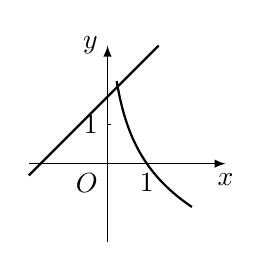
\begin{tikzpicture}[scale = 0.5,>=latex]
    \draw [->] (-2,0) -- (3,0) node [below] {$x$};
    \draw [->] (0,-2) -- (0,3) node [left] {$y$};
    \draw (0,0) node [below left] {$O$};
    \draw (0.1,1) -- (0,1) node [left] {$1$};
    \draw (1,0) node [below] {$1$};
    \draw [thick] (-2,-0.3) -- (1.3,3);
    \draw [thick,domain =-1.1:2.1,samples = 200] plot ({0.5^\x},\x);
\end{tikzpicture}
}{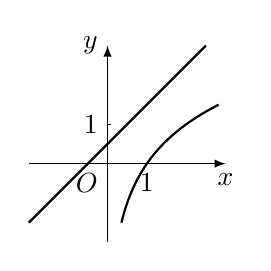
\begin{tikzpicture}[scale = 0.5,>=latex]
    \draw [->] (-2,0) -- (3,0) node [below] {$x$};
    \draw [->] (0,-2) -- (0,3) node [left] {$y$};
    \draw (0,0) node [below left] {$O$};
    \draw (0.1,1) -- (0,1) node [left] {$1$};
    \draw (1,0) node [below] {$1$};
    \draw [thick] (-2,-1.5) -- (2.5,3);
    \draw [thick,domain =1.5:-1.5,samples = 200] plot ({0.5^\x},-\x);
\end{tikzpicture}
}{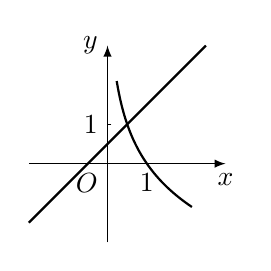
\begin{tikzpicture}[scale = 0.5,>=latex]
    \draw [->] (-2,0) -- (3,0) node [below] {$x$};
    \draw [->] (0,-2) -- (0,3) node [left] {$y$};
    \draw (0,0) node [below left] {$O$};
    \draw (0.1,1) -- (0,1) node [left] {$1$};
    \draw (1,0) node [below] {$1$};
    \draw [thick] (-2,-1.5) -- (2.5,3);
    \draw [thick,domain =-1.1:2.1,samples = 200] plot ({0.5^\x},\x);
\end{tikzpicture}
}{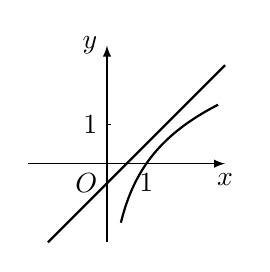
\begin{tikzpicture}[scale = 0.5,>=latex]
    \draw [->] (-2,0) -- (3,0) node [below] {$x$};
    \draw [->] (0,-2) -- (0,3) node [left] {$y$};
    \draw (0,0) node [below left] {$O$};
    \draw (0.1,1) -- (0,1) node [left] {$1$};
    \draw (1,0) node [below] {$1$};
    \draw [thick] (-1.5,-2) -- (3,2.5);
    \draw [thick,domain =1.5:-1.5,samples = 200] plot ({0.5^\x},-\x);
\end{tikzpicture}
}
\item {\tiny (000068)}如果光线每通过一块玻璃其强度要减少$10\%$, 那么至少需要将多少块这样的玻璃重叠起来, 才能使通过它们的光线强度低于原来的$\dfrac 13$?
\item {\tiny (000071)}设$a$为常数且$0<a<1$, 若$y=(\log_a \dfrac 35)^x$在$\mathbf{R}$上是严格增函数, 求实数$a$的取值范围.
\item {\tiny (000075)}仅利用对数函数的单调性和计算器上的乘方功能来确定对数$\log_23$第二位小数的值.
\item {\tiny (000079)}求函数$y=x+\dfrac 4x$的单调区间.
\item {\tiny (000080)}分别作出下列函数的大致图像, 并指出它们的单调区间:\\
(1) $y=|x^2-4x|$;\\
(2) $y=2|x|-3$.
\item {\tiny (000081)}已知二次函数$y=f(x)$, 其中$f(x)=ax^2-2ax+3-a \ (a>0)$. 比较$f(-1)$和$f(2)$的大小.
\item {\tiny (000089)}已知$y=f(x)$是定义在$(-1, 1)$上的奇函数, 在区间$[0, 1)$上是严格减函数, 且$f(1-a)+f(1-a^2)<0$, 求实数$a$的取值范围.
\item {\tiny (000091)}试讨论函数$y=\dfrac{x}{1-x^2}$的单调性.
\item {\tiny (000092)}作出函数$y=(x^2-1)^2-1$的大致图像, 写出它的单调区间, 并证明你的结论.
\item {\tiny (000094)}设函数$y=f(x)$, $x\in \mathbf{R}$的反函数是$y=f^{-1}(x)$.\\
(1) 如果$y=f(x)$是奇函数, 那么$y=f^{-1}(x)$的奇偶性如何?\\
(2) 如果$y=f(x)$在定义域上是严格增函数, 那么$y=f^{-1}(x)$的单调性如何?
\item {\tiny (000355)}有以下命题:\\
\textcircled{1} 若函数$f(x)$既是奇函数又是偶函数, 则$f(x)$的值域为$\{0\}$; \\
\textcircled{2} 若函数$f(x)$是偶函数, 则$f(|x|)=f(x)$;\\
\textcircled{3} 若函数$f(x)$在其定义域内不是单调函数, 则$f(x)$不存在反函数;\\
\textcircled{4} 若函数$f(x)$存在反函数${{f}^{-1}}(x)$, 且${{f}^{-1}}(x)$与$f(x)$不完全相同, 则$f(x)$与${{f}^{-1}}(x)$图像的公共点必在直线$y=x$上; \\
其中真命题的序号是\blank{50}(写出所有真命题的序号).
\item {\tiny (000361)}设$m\in \mathbf{R}$, 若$f(x)=(m+1)x^{\tfrac{2}{3}}+mx+1$是偶函数, 则$f(x)$的单调递增区间是\blank{50}.
\item {\tiny (000434)}已知函数$f(x)=\sin (2x+\dfrac\pi 3)$在区间$[0,a]$(其中$a>0$)上单调递增, 则实数$a$的取值范围是\blank{50}.
\item {\tiny (000445)}已知奇函数$f(x)$是定义在$\mathbf{R}$上的增函数, 数列$\{x_n\}$是一个公差为$2$的等差数列, 满足$f(x_7)+f(x_8)=0$, 则$x_{2017}$的值为\blank{50}.
\item {\tiny (000461)}若从五个数$-1,0,1,2,3$中任选一个数$m$, 则使得函数$f(x)=(m^2-1)x+1$在$\mathbf{R}$上单调递增的概率为\blank{50}(结果用最简分数表示).
\item {\tiny (000498)}已知幂函数的图像过点$(2,\dfrac14)$, 则该幂函数的单调递增区间是\blank{50}.
\item {\tiny (000525)}已知函数$f(x)=\begin{cases} (5-a)x+1, & x<1, \\ a^x, & x\ge 1\end{cases} \ (a>0,a\ne 1)$是实数集$\mathbf{R}$上的增函数, 则实数$a$的取值范围为\blank{50}.
\item {\tiny (000650)}若函数$f(x)=\begin{cases} -x+3a, & x<0,  \\ a^x+1, & x\ge 0 \end{cases}$($a>0$, 且$a\ne 1$)是$\mathbf{R}$上的减函数, 则$a$的取值范围是\blank{50}.
\item {\tiny (001210)}下列函数中, 在$[1,+\infty)$上为增函数的有\blank{50}
\fourch{$y=-(x-1)^2$}{$y=|x-1|$}{$y=\dfrac{1}{x+1}$}{$y=-(x+1)^2$}
\item {\tiny (001211)}求下列各函数的单调区间, 并证明.\\ 
(1) $f(x)=2x+3$;\\ 
(2) $f(x)=\dfrac{1}{x}$;\\ 
(3) $f(x)=x^2+2x$;\\ 
(4) $f(x)=x-\dfrac{1}{x}$;\\ 
(5) $f(x)=ax+\dfrac{b}{x}$, 其中$a>0, \ b>0$;
\item {\tiny (001212)}(1) 设函数$y=f(x)$在区间$I$上单调递增, $x_1,x_2\in I$. 证明$f(x_1)<f(x_2)$当且仅当$x_1<x_2$.\\ 
(2) 已知函数$y=f(x)$是定义在$[-1,1]$上的增函数, 解不等式: $f(x)<f(0)$;\\ 
(3) 已知函数$y=f(x)$是定义在$[-1,1]$上的增函数, 解不等式: $f(x-1)<f(x^2-1)$.
\item {\tiny (001217)}已知$y=f(x)$在$\mathbf{R}$上是增函数.\\ 
\blank{25}(1) 如果$y=g(x)$在区间$I$上递增, 则$y=f(x)+g(x)$在区间$I$上递增;\\ 
\blank{25}(2) 如果$y=g(x)$在区间$I$上递增, 则$y=f(x)g(x)$在区间$I$上递增;\\ 
\blank{25}(3) 如果$y=g(x)$在区间$I$上递增, 则$y=f(g(x))$在区间$I$上递增;\\ 
\blank{25}(4) 如果$y=g(x)$在区间$I$上递增, 则$y=g(f(x))$在$\mathbf{R}$上递增;\\ 
\blank{25}(5) 如果$y=g(x)$满足$y=f(x)-g(x)$在$\mathbf{R}$上递增, 那么$y=g(x)$在$\mathbf{R}$上递减;\\ 
\blank{25}(6) 如果$y=g(x)$满足$y=f(x)-g(x)$在$\mathbf{R}$上递减, 那么$y=g(x)$在$\mathbf{R}$上递减;\\ 
\blank{25}(7) 如果定义在$\mathbf{R}$上的函数$y=g(x)$满足$y=g(f(x))$在$\mathbf{R}$上递增, 则$y=g(x)$在$\mathbf{R}$上递增;\\ 
\blank{25}(8) 如果定义在$\mathbf{R}$上的函数$y=g(x)$满足$y=g(f(x))$在$\mathbf{R}$上递减, 则$y=g(x)$在$\mathbf{R}$上递减.
\item {\tiny (001218)}判断下列各函数的单调性, 并证明.\\ 
(1) $f(x)=\sqrt{1+x}$;\\ 
(2) $f(x)=x+x^5,x\in[0,+\infty)$;\\ 
(3) $f(x)=(\sqrt{x}+1)(x^2+1)$;
\item {\tiny (001222)}是非题, 在每个命题之前的横线上写上``T''或``F''即可, 不用写任何原因.\\ 
已知$y=f(x)$是定义在区间$[-1,1]$上的函数.\\ 
\blank{25}(1) 如果$f(x)$是奇函数, 则$f(x)$要么是增函数, 要么是减函数;\\ 
\blank{25}(2) 如果$f(x)$是偶函数, 则$f(x)$既不是增函数, 又不是减函数;\\ 
\blank{25}(3) 如果$f(x)$是奇函数, 且在$[0,1]$上递增, 那么$f(x)$在$[-1,0]$上也递增;\\ 
\blank{25}(4) 如果$f(x)$是奇函数, 且在$[0,1]$上递增, 那么$f(x)$在$[-1,1]$上也递增;\\ 
\blank{25}(5) 如果$f(x)$在$[-1,0),[-\dfrac{1}{2},\dfrac{1}{2}],(0,1]$上都是递增的, 那么$f(x)$ 在$[-1,1]$上也递增.
\item {\tiny (001223)}是非题, 在每个命题之前的横线上写上``T''或``F''即可, 不用写任何原因.\\ 
已知$y=f(x)$是定义在$[-1,1]$上的偶函数, 在$[0,1]$上递增.\\ 
\blank{25}(1) $f(\dfrac{1}{2})>f(-\dfrac{1}{3})$;\\ 
\blank{25}(2) $f(a)>f(b)$当且仅当$a>b$;\\ 
\blank{25}(3) $f(a)>f(b)$当且仅当$|a|>|b|$;\\ 
\blank{25}(4) $f(a)>f(b)$当且仅当$1\ge |a|>|b|$.
\item {\tiny (001224)}已知函数$f(x)=kx^2-4x+5$在$[1,3]$上单调递减, 则实数$k$的取值范围为\blank{40}.
\item {\tiny (001225)}[选做]
写出函数$f(x)=2x+\dfrac{1}{x^2}$的单调区间, 并证明.
\item {\tiny (001268)}已知函数$y=\dfrac{ax+1}{x+2}$在$(-2,+\infty)$上单调递增, 求$a$的取值范围.
\item {\tiny (001270)}写出下列函数的单调减区间:\\ 
(1) $y=x^2$; \blank{80}\\ 
(2) $y=x^2+2x+3$; \blank{80}\\ 
(3) $y=-x^2+2x+3$; \blank{80}\\ 
(4) $y=\sqrt{-x^2+2x+3}$. \blank{80}
\item {\tiny (001272)}函数$y=x^4-8x^2$的单调增区间为\blank{80}.
\item {\tiny (001273)}已知$y=x^2+2(a-2)x+5$在$[4,+\infty)$上递增, 则实数$a$的取值范围为\blank{50}.
\item {\tiny (001278)}试分析函数$y=x+\sqrt{4-x^2}$的单调性. (提示, 分$x\le0$和$x \ge 0$讨论, 有一部分比较容易)
\item {\tiny (001315)}某地区目前的人口增长率平均为每年$1\%$, 不考虑其他因素, 按这个增长率, 大约经过多少年人口就增加到原来的$2$倍.(精确到$1$年)
\item {\tiny (001319)}已知函数$f(x)=(a^2-1)^x$在$\mathbf{R}$上是减函数, 则实数$a$的取值范围为\blank{80}.
\item {\tiny (001322)}写出下列函数的单调区间和值域(不用证明).\\ 
(1) $y=\left(\dfrac{1}{2}\right)^{x^2+2x+3}$;\\ 
(2) $y=\dfrac{1}{3^x-1}$;\\ 
(3) $y=4^x-2^{x+1}$.
\item {\tiny (001331)}函数$y=\log_{x^2+x-1} 2$的递增区间是\blank{150}.
\item {\tiny (001332)}已知函数$y=f(x)$单调增, 求证:\\ 
(1) 函数$y=f(x)$有反函数$y=f^{-1}(x)$;\\ 
(2) 函数$y=f^{-1}(x)$单调增;
\item {\tiny (001334)}求证: 若递增函数与其反函数的图像有公共点, 则公共点一定在直线$y=x$上.
\item {\tiny (001336)}(1) 写出函数$y=x^{-\frac{4}{3}}$的定义域, 奇偶性, 单调区间;\\ 
(2) 写出函数$y=x^{-\frac{3}{4}}$的定义域, 奇偶性, 单调区间.
\item {\tiny (001337)}作出下列函数的大致图像(只要能够表明定义域和单调性, 凹凸性方面的信息):\\ 
\begin{multicols}{2}
(1) $y=x^{\frac{2}{3}}$; \\ 
(2) $y=x^{-\frac{3}{2}}$; \\ 
\end{multicols}
\begin{multicols}{2}
(3) $y=\dfrac{|x|+1}{|x+1|}$;  \\ 
(4) $y=\dfrac{1}{(x-2)^2}-1$.
\end{multicols}
\item {\tiny (001513)}已知$2$是函数$y=f(x),x\in\mathbf{R}$的周期, 且当$x\in(-1,1]$时, $f(x)=1-x^2$.\\ 
(1) 写出该函数的值域以及所有单调增区间;\\ 
(2) 写出方程$f(x)=\dfrac{1}{2}$的解集;\\ 
(3) 当$x\in(99,101]$时,求$f(x)$的解析式.
\item {\tiny (002827)}已知$y=f(x)$为偶函数, 且$y=f(x)$的图像在$x\in [0,1]$时的部分是半径为$1$的圆弧, 在$x\in [1,+\infty)$时的部分是过点$(2,1)$的射线, 如图.\\
\begin{center}
    \begin{tikzpicture}[>=latex]
        \draw [->] (-1,0) -- (4,0) node [below] {$x$};
        \draw [->] (0,-1) -- (0,3) node [left] {$y$};
        \draw (0,1) arc (90:0:1) -- (3,2);
        \draw (0,0) node [below left] {$O$};
        \draw (1,0) node [below] {$1$};
        \draw (0,1) node [left] {$1$};
        \draw [dashed] (2,0) -- (2,1) -- (0,1);
        \draw (2,0) node [below] {$2$};
    \end{tikzpicture}
\end{center}
(1) 写出函数$y=f(x)$在$x<0$时的单调性:\blank{50};\\
(2) 写出$f(f(-2))$的值:\blank{50};\\
(3) 写出方程$f(x)=\dfrac{\sqrt 3}2$的解集:\blank{50}.
\item {\tiny (002884)}下列函数中, 在其定义域上是单调函数的序号为\blank{50}.\\
\textcircled{1} $y=\dfrac{2-x}x$; \textcircled{2} $y=x-\dfrac 1x$; \textcircled{3} $y={3^{x-1}}$; \textcircled{4} $y=ln\dfrac 1x$; \textcircled{5} $y=tanx$.
\item {\tiny (002885)}函数$y=|x-1|$递减区间的是\blank{50}.
\item {\tiny (002886)}函数$y=x+\dfrac 2x$($x>0$)的递减区间是\blank{50}.
\item {\tiny (002887)}函数$y=(\dfrac 12)^{x^2}$的递减区间是\blank{50}.
\item {\tiny (002888)}函数$y=\dfrac 1{\sqrt{x^2+2x-3}}$的递增区间是\blank{50}.
\item {\tiny (002889)}设常数$a\in \mathbf{R}$.若$y=\dfrac{ax}{x+1}$在区间$(-1,+\infty)$上递增, 则$a$的取值范围是\blank{50}.
\item {\tiny (002890)}设常数$a\in \mathbf{R}$.若函数$y=x^2+ax+1$在$(-\infty,2]$上递减, 则$a$的取值范围是\blank{50}.
\item {\tiny (002891)}若函数$y=f(x)$, $y=g(x)$均为$\mathbf{R}$上增函数, 则下列命题中, 正确的命题的序号是\blank{50}.\\
\textcircled{1} $y=f(x)+g(x)$为增函数; \textcircled{2} $y=f(x)\cdot g(x)$为增函数; \textcircled{3} $y=f(g(x))$为增函数.
\item {\tiny (002892)}若$y=f(x)$为$\mathbf{R}$上的奇函数, 且在$(-\infty,0)$上是减函数, 又$f(-2)=0$, 则$f(x)\le 0$的解集为\blank{50}.
\item {\tiny (002893)}设常数$a\in \mathbf{R}$. 若函数$f(x)=\begin{cases} x+a,& x<1, \\ x^2,& x\ge 1 \end{cases}$在$\mathbf{R}$上递增, 则$a$的取值范围为\blank{50}.
\item {\tiny (002894)}设函数$f(x)=\mathrm{e}^x+\dfrac 1{\mathrm{e}^x}$.\\
(1) 求证: $y=f(x)$在$\mathbf{R}$上不是增函数;\\
(2) 求证: $y=f(x)$在$[0,+\infty)$上是增函数.
\item {\tiny (002895)}设常数$a\in \mathbf{R}$. 若$y=\log_{\frac 12}(x^2-ax+2)$在$[-1,+\infty)$上是减函数, 求$a$的取值范围.
\item {\tiny (002896)}已知定义在区间$(-1,1)$上的函数$y=f(x)$是奇函数, 也是减函数. 若$f(1-a)+f(1-a^2)<0$, 求实数$a$的取值范围.
\item {\tiny (002897)}下列函数中, 在区间$(0 ,+\infty)$上递增的函数的序号为\blank{50}.\\
\textcircled{1} $y=|x+1|$;  \textcircled{2} $y=x-\dfrac 1x$;    \textcircled{3} $y={x^{\frac 12}}$;    \textcircled{4} $y=\sqrt{1-\dfrac 1x}$; \textcircled{5} $y=\lg x$.
\item {\tiny (002899)}已知$y=f(x)$是偶函数, 且在区间$[0,4]$上递减. 记$a=f(2)$, $b=f(-3)$, $c=f(-4)$, 则将$a,b,c$按从小到大的顺序排列是	\blank{50}.
\item {\tiny (002900)}设常数$a\in \mathbf{R}$. ``$a=1$''是``$f(x)=|x-a|$在区间$[1, +\infty)$上为增函数''的\blank{50}条件(填: ``充分不必要''、``必要不充分''、``充要''、``既不充分也不必要''之一).
\item {\tiny (002901)}(1) 设常数$a\in \mathbf{R}$.若函数$y=\dfrac 1{x-a}$在区间$(0,+\infty)$上单调, 则$a$的取值范围为\blank{50}.\\
(2) 设常数$k\in \mathbf{R}$.若函数$f(x)=kx^2-4x+8$在区间$[5,20]$上单调递减, 则$k$的取值范围是\blank{50}.
\item {\tiny (002902)}*设$f(x)$、$g(x)$、$h(x)$是定义域为$R$的三个函数, 对于下列命题:\\
\textcircled{1} 若$f(x)+g(x)$、$f(x)+h(x)$、$g(x)+h(x)$均为增函数, 则$f(x)$、$g(x)$、$h(x)$中至少有一个是增函数;\\
\textcircled{2} 若$f(x)+g(x)$、$f(x)+h(x)$、$g(x)+h(x)$均是以$T$为周期的函数, 则$f(x)$、$g(x)$、$h(x)$均是以$T$为周期的函数, 下列判断正确的是\bracket{20}.
\twoch{\textcircled{1}和\textcircled{2}均为真命题}{\textcircled{1}和\textcircled{2}均为假命题}{\textcircled{1}为真命题, \textcircled{2}为假命题}{\textcircled{1}为假命题, \textcircled{2}为真命题}
\item {\tiny (002903)}设常数$a,b\in \mathbf{R}$. 已知$f(x)=\dfrac{ax^2+1}{x+b}$是奇函数, $f(1)=5$.\\
(1) 求$a,b$的值;\\
(2) 求证: $y=f(x)$在区间$(0,\dfrac 12]$上是减函数.
\item {\tiny (002904)}求证: 函数$f(x)=\dfrac 1x-\lg\dfrac{1+x}{1-x}$是奇函数, 且在区间$(0,1)$上递减.
\item {\tiny (002906)}已知定义$\mathbf{R}$上的函数$y=f(x)$满足下面两个条件:\\
(I) 对于任意$x_1,x_2\in \mathbf{R}$, 都有$f(x_1+x_2)=f(x_1)+f(x_2)$; (II)当$x>0$时, $f(x)>0$, 且$f(1)=1$.\\
(1) 求证: $y=f(x)$是奇函数;\\
(2) 求证: $y=f(x)$在$\mathbf{R}$上是增函数;\\
(3) *解不等式$f(x^2-1)<2$.
\item {\tiny (002908)}下列命题中, 正确的命题的序号是\blank{50}.\\
\textcircled{1} 当$\alpha =0$时, 函数$y={x^{\alpha }}$的图像是一条直线;\\
\textcircled{2} 幂函数的图像都经过(0, 0)和(1, 1)点;\\
\textcircled{3} 当$\alpha <0$且$y={x^{\alpha }}$是奇函数时, 它也是减函数;\\
\textcircled{4} 第四象限不可能有幂函数的图像.
\item {\tiny (002920)}已知函数: \textcircled{1} $y=\dfrac 1x$; \textcircled{2} $y=x^{\dfrac 12}$; \textcircled{3} $y=x^{-\dfrac 12}$; \textcircled{4} $y={x^{\dfrac 23}}$; \textcircled{5} $y=x^{-\dfrac 23}$, 填写分别具有下列性质的函数序号:\\ 
(1) 图像与$x$轴有公共点的:\blank{50};\\
(2) 图像关于原点对称的:\blank{50};\\
(3) 定义域内递减的:\blank{50};\\
(4) 在定义域内有反函数的:\blank{50}.
\item {\tiny (002922)}设$\alpha \in \{-3,-\dfrac 23,-\dfrac 12,-\dfrac 13,\dfrac 13,1,\dfrac 32,2\}$. 已知幂函数$y=x^{\alpha}$是奇函数, 且在区间$(0,+\infty)$上是减函数, 则满足条件的$\alpha$的值是\blank{50}.
\item {\tiny (002923)}下列关于幂函数图像及性质的叙述中, 正确的叙述的序号是\blank{50}.\\
\textcircled{1} 对于一个确定的幂函数, 第二、三象限不可能同时有该幂函数的图像上的点;\\
\textcircled{2} 若某个幂函数图像过$(-1,-1)$, 则该幂函数是奇函数;\\
\textcircled{3} 若某个幂函数在定义域上递增, 则该幂函数图像必经过原点;\\
\textcircled{4} 幂函数图像不会经过点$(-\dfrac 12,8)$以及$(-8,-4)$.
\item {\tiny (002927)}设常数$a,b$满足$a>b>0$. 已知函数$f(x)=\dfrac{x+a}{x+b}$.
(1) 写出函数$y=f(x)$的单调性;\\
(2) 写出函数$y=f(x)$图像的一个对称中心的坐标.
\item {\tiny (002958)}已知函数$f(x)=\dfrac{3^x-3^{-x}}{3^x+3^{-x}}$.\\
(1) 证明$f(x)$在$(-\infty,+\infty)$上是增函数;\\
(2) 求$f(x)$的值域.
\item {\tiny (002960)}已知函数$f(x)=a\cdot 2^x+b\cdot 3^x$, 其中常数$a,b$满足$ab\ne 0$.\\
(1) 若$ab>0$, 判断函数$y=f(x)$的单调性;\\
(2) 若$ab<0$, 求$f(x+1)>f(x)$时$x$的取值范围.
\item {\tiny (002965)}(1) *函数$y=\log_a|x-b|$在$(0,+\infty)$上递增, 则$a$、$b$满足\bracket{20}.
\fourch{$a>1$且$b\ge 0$}{$a>1$且$b\le 0$}{$0<a<1$且$b\ge 0$}{$0<a<1$且$b\le 0$}
(2) 函数$f(x)=\log_a|ax^2-x| \ (a>0,\ a\ne 1)$在区间$[3,4]$上是增函数, 则实数$a$的范围是\blank{50}.
\item {\tiny (002974)}设常数$b\in \mathbf{R}$.若函数$y=x+\dfrac{2^b}x \ (x>0)$在$(0,4]$上是减函数, 在$[4,+\infty)$上是增函数, 则$b=$\blank{50}.
\item {\tiny (002977)}若函数$f(x)=x+\dfrac 4x$($1\le x\le 5$), 则函数$y=f(x)$的递减区间是\blank{50}, 递增区间是\blank{50}, 最小值是\blank{50}, 最大值是\blank{50}.
\item {\tiny (002979)}已知$a>0$, 函数$f(x)=x-\dfrac ax$, 求函数$y=f(x)$的递增区间.
\item {\tiny (002980)}已知函数$y=x+\dfrac ax$有如下性质: 如果常数$a>0$, 那么该函数在$(0, \sqrt a]$上是减函数, 在$[\sqrt a, +\infty)$上是增函数.\\
(1) 设常数$c\in [1,+\infty)$, 求函数$f(x)=x+\dfrac cx \ (1\le x\le 2)$的最大值和最小值;\\
(2) *设常数$c>0$. 当$n$是正整数时, 研究函数$g(x)=x^n+\dfrac c{x^n}$的单调性, 并说明理由.
\item {\tiny (002982)}函数$y=2x+\dfrac 1x$($x<0$)的递增区间是\blank{50}.
\item {\tiny (003000)}已知函数$f(x)=\log_a(x+\sqrt{x^2+1}), \ a>1$.\\
(1) 求$f(x)$的定义域和值域;\\
(2) 求$f^{-1}(x)$;\\
(3) 判断$f^{-1}(x)$的奇偶性、单调性;\\
(4) 若实数$m$满足$f^{-1}(1-m)+f^{-1}(1-m^2)<0$, 求$m$的范围.
\item {\tiny (003002)}设常数$a\in \mathbf{R}$, 区间$E\subseteq (0,+\infty)$. 已知函数$f(x)=\dfrac 1a-\dfrac 1x$, $x\in E$.\\
(1) 求证: $y=f(x)$在区间$E$上递增;\\
(2) 是否存在$a$, 使得对于这样的$a$, 总是存在 $E=[m,n]$($m<n$), 使得$y=f(x)$在区间$E$上的值域也是$E$? 若存在, 求出$a$的取值范围; 若不存在, 说明理由.
\item {\tiny (003601)}下列函数中, 既是奇函数又是减函数的是\bracket{20}.
\fourch{$y=-3x$}{$y=x^3$}{$y=\log_3^x$}{$y=3^x$}
\item {\tiny (003607)}已知某企业今年(2021年)第一季度的营业额为$1.1$亿元, 以后每个季度的营业额比上个季度增加$0.05$亿元, 该企业第一季度的利润为$0.16$亿元, 以后每季度比前一季度增长$4\%$.\\ 
(1) 求2021年起前$20$季度营业额的总和;\\ 
(2) 请问哪一季度的利润首次超过该季度营业额的$18\%$?
\item {\tiny (003625)}命题$p$: 存在$a\in \mathbf{R}$且$a\ne 0$, 对任意的$x\in \mathbf{R}$, 均有$f(x+a)<f(x)+f(a)$恒成立. 已知命题$q_1$: $f(x)$单调递减, 且$f(x)>0$恒成立; 命题$q_2$: $f(x)$单调递增, 且存在${x_0}<0$使得$f({x_0})=0$. 则下列说法正确的是\bracket{20}.
\twoch{$q_1$、$q_2$都是$p$的充分条件}{只有$q_1$是$p$的充分条件}{只有$q_2$是$p$的充分条件}{$q_1$、$q_2$都不是$p$的充分条件}
\item {\tiny (003670)}某群体的人均通勤时间, 是指单日内该群体中成员从居住地到工作地的平均用时. 某地上班族$S$中的成员仅以自驾或公交方式通勤. 分析显示: 当$S$中$x\% \ (0<x<100)$的成员自驾时, 自驾群体的人均通勤时间为
$$f(x)=\begin{cases}
30, & 0<x \le 30,\\ 2x+\dfrac{1800}{x}-90, & 30<x<100\end{cases} \ (\text{单位: 分钟}),$$
而公交群体的人均通勤时间不受$x$影响, 恒为$40$分钟. 试根据上述分析结果回答下列问题:\\
(1) 当$x$在什么范围内时, 公交群体的人均通勤时间少于自驾群体的人均通勤时间;\\
(2) 求该地上班族$S$的人均通勤时间$g(x)$的表达式; 讨论$g(x)$的单调性, 并说明其实际意义.
\item {\tiny (003716)}若函数$f(x)=ax^2+bx+c\ (a>0)$, 不等式$ax^2+bx+c<0$的解集为$\{x|-2<x<0\}$, 当$0<n<m$时, $f(n),f(m),f(\sqrt{mn}),f\left(\dfrac{m+n}2\right)$这四个值中最大的一个是\blank{50}.
\item {\tiny (003801)}下列函数中, 既是偶函数, 又是在区间$(0,+\infty)$上单调递减的函数为\blank{30}.
\fourch{$y=\lg\dfrac{1}{|x|}$}{$y=x^3$}{$y=3^{|x|}$}{$y=x^2$}
\item {\tiny (003884)}已知函数$y=f(x)$的定义域为$\{x|-3\le x\le 8, \ x\ne 5\}$, 值域为$\{y|-1\le y\le 2, \ y\ne 0\}$. 下列关于函数$y=f(x)$的说法: \textcircled{1} 当$x=-3$时, $y=-1$; \textcircled{2} 将$y=f(x)$的图像补上$(5,0)$, 得到的图像必定是一条连续的曲线; \textcircled{3} $y=f(x)$是$[-3,5)$上的单调函数; \textcircled{4} $y=f(x)$的图像与坐标轴只有一个交点. 其中正确的命题是\blank{50}.
\item {\tiny (003966)}(理科)已知函数$f(x)$是定义在$\mathbf{R}$上的单调递减函数且为奇函数, 数列$\{a_n\}$是等差数列, $a_{1007}>0$, 则$f(a_1)+f(a_2)+f(a_3)+\cdots+f(a_{2012})+f(a_{2013})$的值\blank{30}.
\fourch{恒为正数}{恒为负数}{恒为$0$}{可正可负}
\item {\tiny (004005)}求下列函数$y=f(x)$的单调区间和极值点, 其中:
(1) $f(x)=\dfrac 23 x-1$;\\
(2) $f(x)=2+x-x^2$;\\
(3) $f(x)=x^3+x^2-8x+7$.
\item {\tiny (004007)}已知$y=f'(x)$的图像如图所示, 求函数$y=f(x)$在$(-2,2)$上的单调区间和极值点.
\begin{center}
    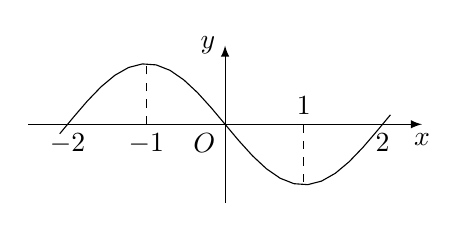
\begin{tikzpicture}[>=latex]
        \draw [->] (-2.5,0) -- (2.5,0) node [below] {$x$};
        \draw [->] (0,-1) -- (0,1) node [left] {$y$};
        \draw (0,0) node [below left] {$O$};
        \draw [domain = -2.1:2.1] plot (\x, {-sin(\x*90)/1.3});
        \draw [dashed] (-1,0) node [below] {$-1$} -- (-1,{1/1.3}) (1,0) node [above] {$1$}-- (1,{-1/1.3});
        \draw (-2,0) node [below] {$-2$} (2,0) node [below] {$2$};
    \end{tikzpicture}
\end{center}
\item {\tiny (004009)}设函数$y=x^3+ax^2+bx+c$的图像与$y=0$在原点相切, 若函数的极小值为$-4$, 求函数的表达式与单调减区间.
\item {\tiny (004013)}讨论函数$y=x^3+ax+b$的单调性(可借助信息技术工具).
\item {\tiny (004094)}已知$f(x)$是定义在$\mathbf{R}$上的奇函数, 对任意两个不相等的正数$x_1$, $x_2$都有$\dfrac{x_2f(x_1)-x_1f(x_2)}{x_1-x_2}<0$, 则函数$g(x)=\begin{cases} \dfrac{f(x)}x, &x\ne 0, \\ 0, & x=0 \end{cases}$\bracket{20}.
\twoch{是偶函数, 且在$(0,+\infty)$上单调递减}{是偶函数, 且在$(0,+\infty)$上单调递增}{是奇函数, 且单调递减}{是奇函数, 且单调递增}
\item {\tiny (004139)}已知常数$a\in \mathbf{R}^+$, 函数$f(x)=3^x+a^2\cdot 3^{-x}$.\\
(1) 若$a=\sqrt{3}$, 解关于$x$的不等式$f(x)<4$;\\
(2) 若$f(x)$在$[3,+\infty)$上为增函数, 求$a$的取值范围.
\item {\tiny (004191)}某种微生物的日增长率为$r$, 经过$n$天后其数量由$p_0$变化为$p$, 并且满足方程$p=p_0\mathrm{e}^{rn}$.实验检测, 这种微生物经过一周数量由$2.58$个单位增长到$14.86$个单位, 则增长率$r=$\blank{50}(精确到$1\%$).
\item {\tiny (004265)}已知a为实数, 函数$f(x)=x|x-a|-a$, $x\in \mathbf{R}$.\\
(1) 当$a=2$时, 求函数$f(x)$的单调递增区间;\\
(2) 若对任意$x\in (0,1)$, $f(x)<0$恒成立, 求a的取值范围.
\item {\tiny (004305)}定义$F(a,b)=\begin{cases} a, & a \le b, \\ b, & a>b,\end{cases}$, 已知函数$f(x)$、$g(x)$定义域都是$\mathbf{R}$, 给出下列命题:\\
(1) 若$f(x)$、$g(x)$都是奇函数, 则函数$F(f(x),g(x))$为奇函数;\\
(2) 若$f(x)$、$g(x)$都是减函数, 则函数$F(f(x),g(x))$为减函数;\\
(3) 若$f_{\min}(x)=m$, $g_{\min}(x)=n$, 则$F_{\min}(f(x),g(x))=F(m,n)$;\\
(4) 若$f(x)$、$g(x)$都是周期函数, 则函数$F(f(x),g(x))$是周期函数.\\
其中正确命题的个数为\bracket{20}.
\fourch{$1$个}{$2$个}{$3$个}{$4$个}
\item {\tiny (004320)}设$a\in \mathbf{R}$. 若函数$y=f(x)$是奇函数, 且$x>0$时, $f(x)=a(x-1)+1$. 若$y=f(x)$是单调增函数, 则$a$取值范围为\blank{50}.
\item {\tiny (004335)}幂函数$y=x^k$的图像经过点$(4,\dfrac 12)$, 则它的单调减区间为\blank{50}.
\item {\tiny (004350)}已知$a$是实常数, $a>0$, $f(x)=ax-1+\dfrac 1{x^2}$.\\
(1) 当$a=2$时, 判断函数$y=f(x)$在区间$[1,+\infty)$上的单调性, 并说明理由;\\
(2) 写出一个$a$的值, 使得$f(x)=0$在区间$(0,+\infty)$上有至少两个不同的解, 并严格证明你的结论.
\item {\tiny (004370)}已知常数$a\in \mathbf{R}^+$, 函数$f(x)=3^x+a^2\cdot 3^{-x}$.\\
(1) 若$a=\sqrt 3$, 解关于$x$的不等式$f(x)<4$;\\
(2) 若$f(x)$在$[3,+\infty)$上为增函数, 求$a$的取值范围.
\item {\tiny (004381)}已知常数$a\in \mathbf{R}$, 函数$f(x)=a\cdot 4^x+2^x+1$在$[3,+\infty)$上单调递减, 则$a$的取值范围为\blank{50}.
\item {\tiny (004386)}已知常数$a\in \mathbf{R}$, 函数$f(x)=ax^2+\lg \dfrac{1+x}{1-x}$.\\
(1) 若$a=0$, 判断$f(x)$的单调性并证明;\\
(2) 问: 是否存在$a$, 使得$f(x)$为奇函数? 若存在, 求出所有$a$的值; 若不存在, 说明理由.
\item {\tiny (004397)}已知函数$f(x)=\begin{cases}  x^2+(4a-3)x+3a,& x<0, \\ \log_a(x+1)+1,& x\ge 0, \end{cases}$($a>0$, $a\ne 1$)在$\mathbf{R}$上单调递减, 且关于$x$的方程$|f(x)|=2-x$恰好有两个不相等的实数解, 则$a$的取值范围是\blank{50}.
\item {\tiny (004423)}设函数$f(x)$是定义在$[a,b]$上的函数, 若存在$x_0\in (a,b)$, 使得$f(x)$在$[a,x_0]$上单调递增, 在$[x_0,b]$上单调递减, 则称$f(x)$为$[a,b]$上的单峰函数, $x_0$称为峰点.\\
(1) 判断下列函数中, 哪些是$[0,2]$上的单峰函数? 若是, 指出峰点; 若不是, 说出原因;\\
\textcircled{1}  $f_1(x)=3x-x^2$; \textcircled{2}  $f_2(x)=\dfrac{2x}{{x^2}+1}$;\\
(2) 若函数$f(x)$是区间$[0,1]$上的单峰函数, 证明: 对任意的$x_1$、$x_2\in (0,1)$, $x_1<x_2$, 若$f(x_1)\ge f(x_2)$, 则峰点在区间$(0,x_2)$内; 若$f(x_1)\le f(x_2)$, 则峰点在区间$(x_1,1)$内.
\item {\tiny (004464)}已知$a$是实常数, 函数$f(x)=a\lg(1-x)-\lg (1+x)$.\\
(1) 若$a=1$, 求证: 函数$y=f(x)$是减函数;\\
(2) 讨论函数$f(x)$的奇偶性, 并说明理由.
\item {\tiny (004525)}已知函数$f(x)=\begin{cases} x^2, & x\text{为无理数}, \\ x, &x\text{为有理数},   \end{cases}$ 则以下$4$个命题:
\textcircled{1} $f(x)$是偶函数; \textcircled{2} $f(x)$在$[0,+\infty)$上是增函数; \textcircled{3} $f(x)$的值域为$\mathbf{R}$; \textcircled{4} 对于任意的正有理数$a$, $g(x)=f(x)-a$存在奇数个零点.
其中正确命题的个数为\bracket{20}.
\fourch{$0$}{$1$}{$2$}{$3$}
\item {\tiny (004530)}已知函数$f(x)$的定义域是$D$, 若对于任意的$x_1,x_2\in D$, 当$x_1<x_2$时, 都有$f(x_1)\le f(x_2)$, 则称函数$f(x)$在$D$上为``非减函数''.\\
(1) 判断$f_1(x)=x^2-4x, \ x\in [1,4]$与$f_2(x)=|x-1|+|x-2|, \ x\in [1,4]$是否是``非减函数''?\\
(2) 已知函数$g(x)=2^x+\dfrac a{2^{x-1}}$在$[2,4]$上为``非减函数'', 求实数$a$的取值范围;\\
(3) 已知函数$h(x)$在$[0,1]$上为``非减函数'', 且满足条件:
\textcircled{1}  $h(0)=0$; \textcircled{2}  $h(\dfrac x3)=\dfrac 12h(x)$; \textcircled{3}  $h(1-x)=1-h(x)$, 求 $h(\dfrac 1{2020})$的值.
\item {\tiny (004569)}改革开放$40$年, 我国卫生事业取得巨大成就, 卫生总费用增长了数十倍. 卫生总费用包括个人现在支出、社会支出、政府支出, 如表为$2012$年至$2015$年我国卫生费用中个人现金支出、社会支出和政府支出的费用(单位:亿元)和在卫生总费用中的占比. 
\begin{center}
    \begin{tabular}{|p{.05\textwidth}<\centering|p{.1\textwidth}<\centering|p{.1\textwidth}<\centering|p{.1\textwidth}<\centering|p{.1\textwidth}<\centering|p{.1\textwidth}<\centering|p{.1\textwidth}<\centering|p{.1\textwidth}<\centering|}
        \hline
         & & \multicolumn{2}{c|}{个人现金卫生支出} & \multicolumn{2}{c|}{社会卫生支出} & \multicolumn{2}{c|}{政府卫生支出} \\ \hline
         年份& 卫生总费用(亿元)& 绝对数(亿元) & 占卫生总费用比重($\%$) & 绝对数(亿元) & 占卫生总费用比重($\%$)& 绝对数(亿元) & 占卫生总费用比重($\%$)\\ \hline
        $2012$ & $28119.00$ & $9656.32$ & $34.34$ & $10030.70$ & $35.67$ & $8431.98$ & $29.99$ \\ \hline
        $2013$ & $31668.95$ & $10729.34$ & $33.88$ & $11393.79$ & $35.98$ & $9545.81$ & $30.14$ \\ \hline
        $2014$ & $35312.40$ & $11295.41$ & $31.99$ & $13437.75$ & $38.05$ & $10579.23$ & $29.96$ \\ \hline
        $2015$ & $40974.64$ & $11992.65$ & $29.27$ & $16506.71$ & $40.29$ & $12475.28$ & $30.45$ \\ \hline
    \end{tabular}
\end{center}
(数据来源于国家统计年鉴)\\
(1) 指出$2012$年到$2015$年之间我国卫生总费用中个人现金支出占比和社会支出占比的变化趋势;\\
(2) 设$t=1$表示$1978$年, 第$t$年卫生总费用与年份$t$之间拟合函数$f(t)=\dfrac{357876.6053}{1+\mathrm{e}^{6.4420-0.1136t}}$, 研究函数$f(t)$的单调性, 并预测我国卫生总费用首次超过$12$万亿的年份.
\item {\tiny (004631)}``函数$y=f(x), \ x\in \mathbf{R}$是增函数''是``函数$y=2-f(x), \ x\in \mathbf{R}$是减函数''的\bracket{20}.
\fourch{充分非必要条件}{必要非充分条件}{充要条件}{既非充分又非必要条件}
\item {\tiny (004679)}为实现``碳达峰'', 减少污染, 某化工企业开发了一个废料回收项目. 经测算, 该项目日回收成本$p$(元)与日回收量$x$(吨)($x\in [0,50]$)的函数关系可表示为$p=\begin{cases}20x, & 0\le x\le 30,  \\ x^2+16x-780, & 30<x \le 50,  \end{cases}$ 且每回收$1$吨废料, 转化成其他产品可收入$80$元.\\
(1) 设日纯收益为$y$元, 写出函数$y=f(x)$的解析式(纯收益$=$收入$-$成本);\\
(2) 该公司每日回收废料多少吨时, 获得纯收益最大?
\item {\tiny (004731)}已知集合$A=\{-2,-1,-\dfrac 12,\dfrac 13,\dfrac 12,1,2,3\}$, 从集合$A$中任取一个元素$a$, 使函数$y=x^a$是奇函数且在$(0,+\infty)$上递增的概率为\blank{50}.
\item {\tiny (004757)}下列函数中既是奇函数, 又在区间$(0,+\infty)$上单调递减的函数为\bracket{20}.
\fourch{$y=\sqrt x$}{$y=\log_{\frac 12}x$}{$y=-x^3$}{$y=x+\dfrac 1x$}
\item {\tiny (004760)}已知以下三个陈述句:\\
$p$: 存在$a\in \mathbf{R}$且$a\ne 0$, 对任意的$x\in \mathbf{R}$, 均有$f(2^{x+a})<f(2^x)+f(a)$恒成立;\\
$q_1$: 函数$y=f(x)$是定义域为$\mathbf{R}$的减函数, 且对任意的$x\in \mathbf{R}$, 都有$f(x)>0$;\\
$q_2$: 函数$y=f(x)$是定义域为$\mathbf{R}$的增函数, 存在$x_0<0$, 使得$f(x_0)=0$;\\
用这三个陈述句组成两个命题, 命题$S$: ``若$q_1$, 则$p$''; 命题$T$: ``若$q_2$, 则$p$''. 关于$S,T$以下说法正确的是\bracket{20}.
\twoch{只有命题$S$是真命题}{只有命题$T$是真命题}{两个命题$S,T$都是真命题}{两个命题$S,T$都不是真命题}
\item {\tiny (004763)}新冠肺炎疫情造成医用防护服紧缺, 某地政府决定为防护服生产企业A公司扩大生产提供$x$($x\in [0,10]$)(万元)的专项补贴, 并以每套$80$元的价格收购其生产的全部防护服. $A$公司在收到政府$x$(万元)补贴后, 防护服产量将增加到$t=k\cdot (6-\dfrac{12}{x+4})$(万套), 其中$k$为工厂工人的复工率($k\in [0.5,1]$). $A$公司生产$t$万件防护服还需投入成本$20+8x+50t$(万元).\\
(1) 将$A$公司生产防护服的利润$y$(万元)表示为补贴$x$(万元)的函数(利润不包含政府补贴);\\
(2) 若对任意的$x\in [0,10]$(万元), $A$公司都不会产生亏损, 求复工率$k$的取值范围.
\item {\tiny (005052)}利用函数的单调性证明: 若$x>0$, $y>0$, $x+y=1$, 则$(x+\dfrac 1x)(y+\dfrac 1y)\ge \dfrac{25}4$.
\item {\tiny (005053)}利用函数的单调性证明: 若$0<a<\dfrac 1k(k\ge 2,k\in \mathbf{N})$, 且$a^2<a-b$, 则$b<\dfrac 1{k+1}$.
\item {\tiny (005253)}已知常数$a\in (0,1)$, 对任意$x>0$, $f(\log_ax)=\dfrac{a(x^2-1)}{x(a^2-1)}$.\\
(l) 求$f(x)$($x\in \mathbf{R}$)的表达式, 并判断它的单调性;\\
(2) 若$n\ge 2$, $n\in \mathbf{N}$, 求证: $f(n)>n$.
\item {\tiny (005357)}将进货单价为$40$元的商品按每件$50$元出售时, 每月能卖出$500$个, 已知这批商品在销售单价的基础上每涨价$1$元, 其月销售数就减少$10$个, 为了每月赚取最大利润, 销售单价应定为多少?
\item {\tiny (005359)}求证: 函数$f(x)=x^3$在$x\in \mathbf{R}$上是增函数.
\item {\tiny (005360)}已知奇函数$y=f(x)$在$x<0$时是减函数, 求证: $y=f(x)$在$x>0$时也是减函数.
\item {\tiny (005362)}已知函数$y=f(x)$满足$f(x)=f(4-x)$($x\in \mathbf{R}$), 且$f(x)$在$x>2$时为增函数, 记$a=f(\dfrac 35)$, $b=f(\dfrac 65)$, $c=f(4)$, 则$a,b,c$之间的大小关系是\bracket{20}.
\fourch{$c>a>b$}{$c>b>a$}{$b>a>c$}{$a>c>d$}
\item {\tiny (005472)}函数$y=\sqrt {x^2+2x-3}$为减函数的区间是\bracket{20}.
\fourch{$(-\infty ,-3]$}{$[-1,+\infty)$}{$(-\infty ,-1]$}{$[1,+\infty)$}
\item {\tiny (005473)}若函数$y=(2k+1)x+b$在$(-\infty,+\infty)$上是减函数, 则\bracket{20}.
\fourch{$k>\dfrac 12$}{$k<\dfrac 12$}{$k>-\dfrac 12$}{$k<-\dfrac 12$}
\item {\tiny (005474)}若函数$f(x)=4x^2-mx+5$在区间$[-2,+\infty)$上是增函数, 在区间$(-\infty ,-2]$上是减函数, 则$f(1)$等于\bracket{20}.
\fourch{$-7$}{$1$}{$17$}{$25$}
\item {\tiny (005475)}若函数$y=x^2+2(a-2)x+5$在区间$(4,+\infty)$上是增函数, 则实数$a$的取值范围是\bracket{20}.
\fourch{$a\le -2$}{$a\ge -2$}{$a\le -6$}{$a\ge -6$}
\item {\tiny (005476)}下列函数中, 在区间$(0,2)$上为增函数的是\bracket{20}.
\fourch{$y=-3x+1$}{$y=\sqrt[3]x$}{$y=x^2-4x+3$}{$y=\dfrac 4x$}
\item {\tiny (005477)}若函数$f(x)$在定义域$\mathbf{R}$上为增函数, 且$f(x)<0$, 则下列函数在$\mathbf{R}$上为增函数的是\bracket{20}.
\fourch{$y=|f(x)|$}{$y=\dfrac 1{f(x)}$}{$y=[ f(x) ]^2$}{$y=[ f(x) ]^3$}
\item {\tiny (005478)}函数$y=\dfrac 1{\sqrt {x^2-4x+5}}$为增函数的区间是\blank{50}, 为减函数的区间是\blank{50}.
\item {\tiny (005479)}函数$y=\dfrac 1{\sqrt {3+2x-x^2}}$为增函数的区间是\blank{50}.
\item {\tiny (005480)}函数$y=|3x-5|$为减函数的区间是\blank{50}.
\item {\tiny (005481)}函数$y=|x^2-2x-3|$为增函数的区间是\blank{50}.
\item {\tiny (005482)}函数$y=\dfrac{1-x}{1+x}$为减函数的区间是\blank{50}.
\item {\tiny (005483)}定义在$[1, 3]$上的函数$f(x)$为减函数, 求满足不等式$f(1-a)-f(3-a^2)>0$的解集.
\item {\tiny (005484)}已知$f(x)=-x^3-x+1$($x\in \mathbf{R}$), 求证$y=f(x)$在定义域上为减函数.
\item {\tiny (005485)}求证: 函数$f(x)=x+\dfrac 1x$在$(0, 1)$上是减函数, 在$(1,+\infty)$上是增函数.
\item {\tiny (005486)}求证: $f(x)=\sqrt x-\dfrac 1x$在定义域上是增函数.
\item {\tiny (005487)}已知常数$m,n$满足$mn<2$, 求证: 函数$f(x)=\dfrac{mx+1}{2x+n}$在$(-\dfrac n2,+\infty)$上为减函数.
\item {\tiny (005488)}已知$f(x)=x^2+1$, $g(x)=x^4+2x^2+2$, 是否存在实数$\lambda$, 使得$F(x)=g(x)-\lambda f(x)$在$(-\infty ,-1)$上是减函数, 在$(-1,0)$上是增函数? 说明理由.
\item {\tiny (005489)}已知函数$f(x)$在区间$(-\infty ,+\infty)$上是增函数, 又实数$a,b$满足$a+b\ge 0$, 求证: $f(a)+f(b)\ge f(-a)+f(-b)$.
\item {\tiny (005490)}$f(x)$是定义在$\mathbf{R}^+$的增函数, 且$f(\dfrac xy)=f(x)-f(y)$.\\
(1) 求$f(1)$的值;\\
(2) 若$f(6)=1$, 解不等式$f(x+3)-f(\dfrac 1x)<2$.
\item {\tiny (005491)}若$f(x)=(m-1)x^2+3mx+3$为偶函数, 则$f(x)$在区间$(-4,2)$上\bracket{20}.
\twoch{是增函数}{是减函数}{先是增函数后是减函数}{先是减函数后是增函数}
\item {\tiny (005493)}下列函数中既是奇函数, 又在定义域上为增函数的是\bracket{20}.
\fourch{$f(x)=3x+1$}{$f(x)=\dfrac 1x$}{$f(x)=1-\dfrac 1x$}{$f(x)=x^3$}
\item {\tiny (005499)}若奇函数$f(x)$在区间$[-3, -1]$上是增函数, 且有最大值$-2$, 则$f(x)$在$[1, 3]$上是\blank{50}函数(填``增''或``减''), 且最小值等于\blank{50}.
\item {\tiny (005500)}设$f(x)$为定义在$\mathbf{R}$上的偶函数, 且$f(x)$在$[0,+\infty)$上是增函数, 则$f(-4)$, $f(-2)$, $f(3)$由小到大的排列顺序为\blank{50}.
\item {\tiny (005503)}若函数$f(x)=8+2x-x^2$, 记$g(x)=f(2-x^2)$, 则$g(x)$\bracket{20}.
\fourch{在(-2, 0)上是增函数}{在(0, 2)上是增函数}{在(-1, 0)上是减函数}{在(0, 1)上是减函数}
\item {\tiny (005504)}函数$f(x)=x|x|-2x$是\bracket{20}.
\twoch{偶函数, 且在(-1, 1)上是增函数}{奇函数, 且在(-1, 1)上是减函数}{偶函数, 且在(-1, 1)上是减函数}{奇函数, 且在(-1, 1)上是增函数}
\item {\tiny (005519)}已知奇函数$f(x)$在定义域$(-l, l)$上是减函数, 求满足$f(1-m)+f(1-m^2)<0$的实数$m$的取值范围.
\item {\tiny (005520)}已知偶函数$f(x)$在$[0,+\infty)$上是增函数.求不等式$f(2x+5)<f(x^2+2)$的解集.
\item {\tiny (005541)}已知函数$f(x)=\dfrac{x+1}{x-1}$, $g(x)=f^{-1}(-x)$, 则$g(x)$\bracket{20}.
\twoch{在$(-\infty ,+\infty)$上是增函数}{在$(-\infty ,-1)$上是增函数}{在$(1,+\infty)$上是减函数}{在$(-\infty ,-1)$上是减函数}
\item {\tiny (005559)}求函数$y=(\dfrac 12)^{-x^2+2x}$为增函数的区间.
\item {\tiny (005561)}填写下表:
\begin{center}
    \begin{tabular}{|c|c|c|c|c|}
        \hline
        $x$	 & $f(x)=x^2$ & $f(x)-f(x-1)$ & $g(x)=2^x$ & $g(x)-g(x-1)$ \\ \hline
        $0$ & & & & \\ \hline
        $1$ & & & & \\ \hline
        $2$ & & & & \\ \hline
        $3$ & & & & \\ \hline
        $4$ & & & & \\ \hline
        $5$ & & & & \\ \hline
        $6$ & & & & \\ \hline
        $7$ & & & & \\ \hline
        $8$ & & & & \\ \hline
        $9$ & & & & \\ \hline
        $10$ & & & & \\ \hline
    \end{tabular}
\end{center}
(1) 比较$f(x)=x^2$与$g(x)=2^x$的函数值的大小;\\
(2) 比较$f(x)=x^2$与$g(x)=2^x$的函数值递增的快慢.
\item {\tiny (005562)}已知函数$f(x)=2x+1$, $g(x)=1.5^x$, $h(x)=x^{1.5}$, 试用数值计算比较三个函数在$[0,+\infty)$上的函数值的大小、图像递增的快慢. 并说明在函数图像上的表现.
解  列表并计算得:
\begin{center}
    \begin{longtable}{|c|c|c|c|c|c|c|}
        \hline
        $x$	 & $f(x)=2x+1$ & $f(x)-f(x-1)$ & $g(x)=1.5^x$ & $g(x)-g(x-1)$ & $h(x)=x^{1.5}$ & $h(x)-h(x-1)$ \\ \hline
        \endhead
        $0$ & $1$ & & $1$ & & $0$ &  \\ \hline
        $1$ & $3$ & $2$ & $1.5$ & $0.5$ & $1$ & $1$\\ \hline
        $2$ & $5$ & $2$ & $2.25$ & $0.75$ & $2.82842712$ & $1.82842712$\\ \hline
        $3$ & $7$ & $2$ & $3.375$ & $1.125$ & $5.19615242$ & $2.3677253$\\ \hline
        $4$ & $9$ & $2$ & $5.0625$ & $1.6875$ & $8$ & $2.80384758$\\ \hline
        $5$ & $11$ & $2$ & $7.59375$ & $2.53125$ & $11.1803399$ & $3.18033989$\\ \hline
        $6$ & $13$ & $2$ & $11.390625$ & $3.796875$ & $14.6969385$ & $3.51659857$\\ \hline
        $7$ & $15$ & $2$ & $17.085938$ & $5.6953125$ & $18.5202592$ & $3.82332072$\\ \hline
        $8$ & $17$ & $2$ & $25.628906$ & $8.5429688$ & $22.627417$ & $4.10715782$\\ \hline
        $9$ & $19$ & $2$ & $38.443359$ & $12.814453$ & $27$ & $4.372583$\\ \hline
        $10$ & $21$ & $2$ & $57.665039$ & $19.22168$ & $31.6227766$ & $4.6227766$\\ \hline
        $11$ & $23$ & $2$ & $86.497559$ & $28.83252$ & $36.4828727$ & $4.86009609$\\ \hline
        $12$ & $25$ & $2$ & $129.74634$ & $43.248779$ & $41.5692194$ & $5.08634669$\\ \hline
        $13$ & $27$ & $2$ & $194.61951$ & $64.873169$ & $46.8721666$ & $5.3029472$\\ \hline
        $14$ & $29$ & $2$ & $291.92926$ & $97.309753$ & $52.3832034$ & $5.51103683$\\ \hline
        $15$ & $31$ & $2$ & $437.89389$ & $145.96463$ & $58.0947502$ & $5.71154678$\\ \hline
        $16$ & $33$ & $2$ & $656.84084$ & $218.94695$ & $64$ & $5.90524981$\\ \hline
        $17$ & $35$ & $2$ & $985.26125$ & $328.42042$ & $70.0927956$ & $6.09279564$\\ \hline
        $18$ & $37$ & $2$ & $1477.8919$ & $492.63063$ & $76.3675324$ & $6.27473673$\\ \hline
        $19$ & $39$ & $2$ & $2216.8378$ & $738.94594$ & $82.8190799$ & $6.45154756$\\ \hline
        $20$ & $41$ & $2$ & $3325.2567$ & $1108.4189$ & $89.4427191$ & $6.62363917$\\ \hline
        $21$ & $43$ & $2$ & $4987.8851$ & $1662.6284$ & $96.2340896$ & $6.79137049$\\ \hline
        $22$ & $45$ & $2$ & $7481.8276$ & $2493.9425$ & $103.189147$ & $6.95505712$\\ \hline
        $23$ & $47$ & $2$ & $11222.741$ & $3740.9138$ & $110.304125$ & $7.11497832$\\ \hline
        $24$ & $49$ & $2$ & $16834.112$ & $5611.3707$ & $117.575508$ & $7.27138262$\\ \hline
        $25$ & $51$ & $2$ & $25251.168$ & $8417.0561$ & $125$ & $7.42449235$\\ \hline
        $26$ & $53$ & $2$ & $37876.752$ & $12625.584$ & $132.574507$ & $7.57450735$\\ \hline
        $27$ & $55$ & $2$ & $56815.129$ & $18938.376$ & $140.296115$ & $7.72160806$\\ \hline
        $28$ & $57$ & $2$ & $85222.693$ & $28407.564$ & $148.162073$ & $7.86595801$\\ \hline
        $29$ & $59$ & $2$ & $127834.04$ & $42611.346$ & $156.169779$ & $8.00770599$\\ \hline
        $30$ & $61$ & $2$ & $191751.06$ & $63917.02$ & $164.316767$ & $8.14698784$\\ \hline
        $\cdots$ & $\cdots$ & $\cdots$ & $\cdots$ & $\cdots$ & $\cdots$ & $\cdots$ \\ \hline
    \end{longtable}
\end{center}
得点$A,B,C,D$的横坐标分别约为$1.5,4.8, 6.5, 7.4$, 记作$x_A,x_B,x_C,x_D$.\\
(1) 三个函数的函数值的大小情况如下:\\
\textcircled{1} 当$0<x<x_A$时, $f(x)>g(x)>h(x)$;
\textcircled{2} 当$x_A<x<x_B$时, $f(x)>h(x)>g(x)$;
\textcircled{3} 由$x_B<x<x_C$时, $h(x)>f(x)>g(x)$;
\textcircled{4} 当$x_C<x<x_D$时, $h(x)>g(x)>f(x)$;
\textcircled{5} 当$x_D<x$时, $g(x)>h(x)>f(x)$;
\textcircled{6} 当$x=x_A$时, $f(x)>g(x)=h(x)$;
\textcircled{7} 当$x=x_B$时, $f(x)=h(x)>g(x)$;
\textcircled{8} 当$x=x_C$时, $f(x)=g(x)<h(x)$;
\textcircled{9} 当$x=x_D$时, $f(x)<g(x)=g(x)$.\\
(2) 它们在同一个平面直角坐标系下的图像如图14所示.
\begin{center}
    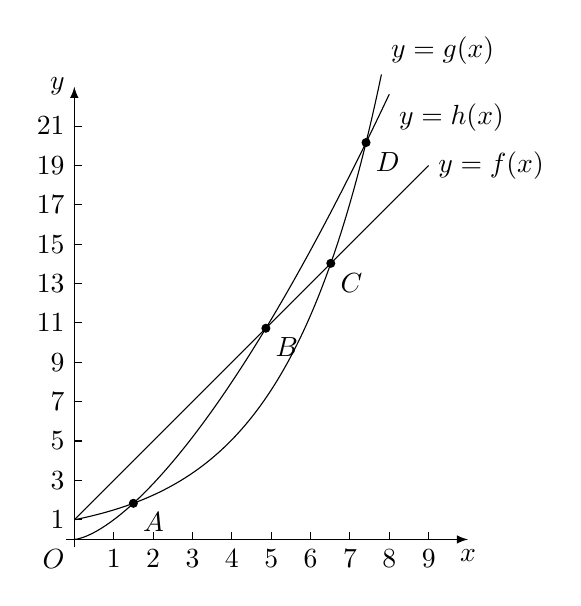
\begin{tikzpicture}[>=latex]
        \draw [->] (-0.1,0) -- (5,0) node [below] {$x$};
        \draw [->] (0,-0.1) -- (0,5.75) node [left] {$y$};
        \draw (0,0) node [below left] {$O$};
        \draw [domain = 0:9,samples = 100, name path = firstorder] plot ({\x/2},{(2*\x+1)/4});
        \draw (4.5,{19/4}) node [right] {$y=f(x)$};
        \draw [domain = 0:7.8, samples = 100, name path = exponential] plot ({\x/2},{1.5^(\x)/4}); 
        \draw (3.9,{1.5^7.8/4}) node [above right] {$y=g(x)$};
        \draw [domain = 0:8, samples = 100, name path = power] plot ({\x/2},{\x^(3/2)/4});
        \draw (4,{8^(3/2)/4}) node [below right] {$y=h(x)$};
        \path [name intersections = {of = firstorder and exponential, by = {T,C}}];
        \path [name intersections = {of = firstorder and power, by = B}];
        \path [name intersections = {of = exponential and power, by = {A,D}}];
        \filldraw (A) circle (0.05) node [below right] {$A$};
        \filldraw (B) circle (0.05) node [below right] {$B$};
        \filldraw (C) circle (0.05) node [below right] {$C$};
        \filldraw (D) circle (0.05) node [below right] {$D$};
        \foreach \i in {1,2,...,9}{\draw (\i/2,0.1) -- (\i/2,0) node [below] {$\i$};};
        \foreach \i in {1,3,...,21}{\draw (0.1,\i/4) -- (0,\i/4) node [left] {$\i$};};
    \end{tikzpicture}
\end{center}
由表格及图像可看出, 三个函数的函数值变化及相应增量规律为: 随着$x$的增大, 直线型均匀上升, 增量恒定; 指数型急剧上升, 在区间$[0,+\infty)$上递增增量快速增大; 幂函数型虽上升较快, 但随着$x$的不断增大上升趋势远不如指数型, 几乎微不足道, 其增量缓慢递增.
\item {\tiny (005571)}若$f(x)$在$(0,+\infty)$上是减函数, 而$f(a^x)$在$(-\infty ,+\infty)$上是增函数, 则实数$a$的取值范围是\bracket{20}.
\fourch{(0, 1)}{$(0,1)\cup (1,+\infty)$}{$(0,+\infty)$}{$(1,+\infty)$}
\item {\tiny (005572)}函数$y=(\dfrac 12)^{\sqrt {-x^2+x+x}}$为增函数的区间是\bracket{20}.
\fourch{$[-1,\dfrac 12]$}{$(-\infty ,-1]$}{$[2,+\infty)$}{$[\dfrac 12,2]$}
\item {\tiny (005573)}若函数$f(x)=(a^2-1)^x$在$(-\infty ,+\infty)$上是减函数, 则$a$的取值范围是\bracket{20}.
\fourch{$|a|>1$}{$|a|<\sqrt 2$}{$a>\sqrt 2$}{$1<|a|<\sqrt 2$}
\item {\tiny (005580)}函数$y=3^{x^2-3x-2}$为增函数的区间是\blank{50}.
\item {\tiny (005581)}函数$y=(0.2)^{x^2-6x+9}$为增函数的区间是\blank{50}.
\item {\tiny (005582)}函数$y=2^{-|x|}$为增函数的区间是\blank{50}.
\item {\tiny (005583)}函数$y=(\dfrac 12)^{|1+2x|}$为增函数的区间是\blank{50}, 为减函数的区间是\blank{50}.
\item {\tiny (005584)}若函数$y=(\dfrac 12)^{(m^2-1)x}$在$x\in \mathbf{R}$为减函数, 则实数$m$的取值范围是\blank{50}.
\item {\tiny (005597)}已知$f(x)=\dfrac{a^x-1}{a^x+1}$($a>1$).\\
(1) 判断函数$f(x)$的奇偶性;\\
(2) 求函数$f(x)$的值域;\\
(3) 求证: $f(x)$在区间$(-\infty ,+\infty)$上是增函数.
\item {\tiny (005600)}已知函数$f(x)=\dfrac a{a^2-2}(a^x-a^{-x})$($a>0$且$a\ne 1$)在$(-\infty ,+\infty)$上是增函数, 求实数$a$的取值范围.
\item {\tiny (005605)}在同一个平面直角坐标系中, 作出$t(x)=0.5x$与$g(x)=0.2\times 2^x$的图像, 并比较它们的增长情况.
\item {\tiny (005607)}用计算器计算并填写下表:
\begin{center}
    \begin{tabular}{|c|c|c|c|c|}
        \hline
        $x$	& $f(x)=x^{\frac 12}$ & $g(x)=x^{0.6}$ & $h(x)=2.1^x$ & $s(x)=2.2^x$ \\ \hline
        $0$ & & & & \\ \hline
        $1$ & & & & \\ \hline
        $2$ & & & & \\ \hline
        $3$ & & & & \\ \hline
        $4$ & & & & \\ \hline
        $5$ & & & & \\ \hline
        $6$ & & & & \\ \hline
        $7$ & & & & \\ \hline
        $8$ & & & & \\ \hline
        $9$ & & & & \\ \hline
        $10$ & & & & \\ \hline
    \end{tabular}
\end{center}
从表中变化的现象可以归纳出哪些函数递增的规律?\\
(1) 幂函数$f(x)$与$g(x)$之间比较得出的规律;
(2) 指数函数$h(x)$与$s(x)$之间比较得出的规律;
(3) 幂函数$f(x)=x^{\frac 12}$与指数函数$h(x)$之间比较得出的规律
\item {\tiny (005684)}求函数$f(x)=\log_{0.2}(x-1)(x+2)$为增函数的区间.
\item {\tiny (005691)}设$f(x)$是定义在$(-\infty ,+\infty)$上的偶函数, 且它在$[0,+\infty)$上是增函数, 记$a=f(-\log_{\sqrt 2}\sqrt 3)$, $b=f(-\log_{\sqrt 3}\sqrt 2)$, $c=f(-2)$, 则$a,b,c$的大小关系是\bracket{20}.
\fourch{$a>b>c$}{$b>c>a$}{$c>a>b$}{$c>b>a$}
\item {\tiny (005703)}函数$y=\log_{\frac 13}(x^2-5x+6)$为减函数的区间是\blank{50}.
\item {\tiny (005704)}函数$y=\lg (12-4x-x^2)$为增函数的区间是\blank{50}.
\item {\tiny (005705)}函数$y=-\log_{\frac 12}(-x)$为减函数的区间是\blank{50}.
\item {\tiny (005706)}若函数$y=\log_a(1-x)$在$[0,1)$上是增函数, 则$a$的取值范围是\blank{50}.
\item {\tiny (005707)}函数$y=\log_{\frac 12}^2x-\log_{\frac 12}x+1$为增函数的区间是\blank{50}.
\item {\tiny (005713)}函数$y=\lg \dfrac{1-x}{1+x}$\bracket{20}.
\twoch{是奇函数, 且在$(-1, 1)$是增函数}{是奇函数, 且在$(-1, 1)$上是减函数}{是偶函数, 且在$(-1, 1)$是增函数}{是偶函数, 且在$(-1, 1)$上是减函数}
\item {\tiny (005716)}已知$f(x)=\dfrac{a^x-1}{a^x+1}$($a>1$).\\
(1) 求$f(x)$的值域;\\
(2) 求证: $f(x)$在$R$上是增函数;\\
(3) 求$f(x)$的反函数.
\item {\tiny (005717)}已知$f(\log_ax)=\dfrac{a(x^2-1)}{x(a^2-1)}$($x>0$, $0<a<1$), 求证: 函数$f(x)$在$(-\infty ,+\infty)$上是增函数.
\item {\tiny (005718)}若函数$f(x)=\log_a|x+1|$在$(-1, 0)$上有$f(x)>0$, 则$f(x)$\bracket{20}.
\twoch{在$(-\infty ,0)$上是增函数}{在$(-\infty ,0)$是减函数}{在$(-\infty ,-1)$上是增函数}{在$(-\infty ,-1)$是减函数}
\item {\tiny (005741)}已知$f(x)=\log_a|\log_ax|$($0<a<1$).\\
(1) 解不等式: $f(x)>0$;\\
(2) 判断$f(x)$在$(1,+\infty)$上的单调性, 并证明之.
\item {\tiny (005743)}已知函数$f(x)=\sqrt {\log_ax-1}$($a>0$且$a\ne 1$).\\
(1) 求$f(x)$的定义域;\\
(2) 当$a>1$时, 求证: $f(x)$在$[a,+\infty)$上是增函数.
\item {\tiny (005749)}已知函数$f(x)=\log_{\frac 12}(x^2-2x)$.\\
(1) 求它的单调区间;\\
(2) 求$f(x)$为增函数时的反函数.
\item {\tiny (005750)}已知函数$f(x)=\log_a\dfrac{x+b}{x-b}$($a>0$, $b>0$且$a\ne 1$).\\
(1) 求$f(x)$的定义域;\\
(2) 讨论$f(x)$的奇偶性;\\
(3) 讨论$f(x)$的单调性;\\
(4) 求$f(x)$的反函数$f^{-1}(x)$.
\item {\tiny (005808)}已知函数$f(x)=x^2-x+k$满足$\log_2f(a)=2$, $f(\log_2a)=k$($a>0$且$a\ne 1$), 求$f(\log_2x)$在什么区间上是减函数, 并求出$a$与$k$的值.
\item {\tiny (005832)}已知函数$f(x)$($x\ne 0$)满足$f(xy)=f(x)+f(y)$.
(1) 求证: $f(1)=f(-1)=0$;\\
(2) 求证: $f(x)$为偶函数;\\
(3) 若$f(x)$在$(0,+\infty)$上是增函数, 解不等式$f(x)+f(x-\dfrac 12)\le 0$.
\item {\tiny (005833)}已知函数$f(x)$对一切实数$x,y$满足$f(0)\ne 0$, $f(x+y)=f(x)\cdot f(y)$, 且当$x<0$时, $f(x)>1$.求证:
(1)当$x>0$时, $0<f(x)<1$.
(2)$f(x)$在$x\in \mathbf{R}$上是减函数.
\item {\tiny (005841)}已知$y=f(x)$在其定义域上是增函数, 求证: $y=f(x)$的反函数$y=f^{-1}(x)$在其定义域上也是增函数.
\item {\tiny (005842)}已知函数$f(x)=x^3+x+1$($x\in \mathbf{R}$), 求证:\\
(1) $f(x)$是$\mathbf{R}$上的增函数;\\
(2) 方程$x^3+x+1=0$只有一个实数解.
\item {\tiny (005843)}已知函数$f(x)=\dfrac x{1+x^2}$($x\in \mathbf{R}$).\\
(1) 求$f(x)$的值域;\\
(2) 讨论$f(x)$的单调性.
\item {\tiny (005855)}已知$f(x)$在$(-\infty ,+\infty)$上有单调性, 且满足$f(1)=2$和$f(x+y)=f(x)+f(y)$.\\
(1) 求证: $f(x)$为奇函数;\\
(2) 若$f(x)$满足$f(k\log_2t)+f(\log_2t-\log_2^2t-2)<0$, 求实数$k$的取值范围.
\item {\tiny (005856)}已知函数$f(x)$在定义域$x\in \mathbf{R}^+$上是增函数, 且满足$f(x\cdot y)=f(x)+f(y)$($x,y\in \mathbf{R}^+$).\\
(1) 求$f(x)$在$(1,+\infty)$上的值域;\\
(2) 若$f(2)=1$, $f(x)$图像上三点$A,B,C$的横坐标分别为$a,a+2,a+4$($a>0$), 且$\triangle ABC$的面积小于$1$, 求实数$a$的取值范围.
\item {\tiny (007873)}为分流短途乘客, 减缓轨道交通高峰压力, 上海地铁实行新的计费标准. 新标准的分段计程制度如下: $0-6$千米(含$6$千米)$3$元; $6-16$千米(含$16$千米)$4$元; $16$千米以上每$6$千米递增$1$元, 但总票价不超过$8$元.\\
(1) 试作出票价$y$(元)关于路程$x$(千米)的函数图像;\\
(2) 某人买了$5$元的车票, 他途经路程不能超过多少千米?
\item {\tiny (007899)}已知函数$y=f(x)$的定义域为$[0,+\infty)$.如果对任意的$x>0$, 都有$f(x)<f(0)$, 那么函数$y=f(x)$有$[0,+\infty)$上是否一定是减函数?
\item {\tiny (007900)}求证: 函数$f(x)=x-\dfrac 1x,x\in (-\infty ,0)$是增函数.
\item {\tiny (007901)}判断函数$f(x)=2x+\dfrac 2x,x\in [\dfrac 12,3]$的单调性, 并求出它的单调区间.
\item {\tiny (007902)}如果函数$y=x^2-2mx+1$在$(-\infty ,2]$上是减函数, 那么实数$m$的取值范围是\blank{50}.
\item {\tiny (007903)}当函数$f(x)=$\blank{50}时, 函数$f(x)$同时满足条件: \textcircled{1} 函数$f(x)$不是偶函数; \textcircled{2} 在区间$(-\infty ,-1)$上是减函数; \textcircled{3} 在区间$(0,1)$上是增函数(写出一个你认为正确的函数解析式).
\item {\tiny (007911)}画出函数$y=x^2-2|x|$的图像, 并写出它的定义域、奇偶性、单调区间、最小值.
\item {\tiny (007912)}研究函数$f(x)=\dfrac 1{1+x^2}$的定义域、奇偶性、单调性、最大值.
\item {\tiny (007916)}已知$a\ne 0$, 试讨论函数$f(x)=\dfrac a{1-x^2}$在区间$(0,1)$上的单调性.
\item {\tiny (007923)}研究函数$f(x)=x+\dfrac ax(a>0)$的定义域、奇偶性、单调性.
\item {\tiny (007930)}已知函数$f(x)=x$, $g(x)=-\dfrac 4x$, $p(x)=f(x)-g(x)$, 求$y=p(x)$的函数表达式, 并写出$y=p(x)$的单调递减区间.
\item {\tiny (007931)}作出函数$y=|x^2-4x|$的图像, 并指出其单调区间.
\item {\tiny (007932)}作出函数$y=2|x|-3$的图像, 并指出其单调区间.
\item {\tiny (007939)}已知$y=f(x)$是定义在$(-1,1)$上的奇函数, 在区间$[0,1)$上是减函数, 且$f(1-a)+f(1-a^2)<0$, 求实数$a$的取值范围.
\item {\tiny (007941)}已知函数$y=f(x)$具有如下性质:\\
\textcircled{1} 定义在$\mathbf{R}$上的偶函数; \textcircled{2} 在$(-\infty ,0)$上为增函数; \textcircled{3} $f(0)=1$; \textcircled{4} $f(-2)=-7$; \textcircled{5} 不是二次函数.\\
求$y=f(x)$的一个可能的解析式.
\item {\tiny (007942)}打开水龙头, 让水匀速地注入一个杯子内, 随着时间的增加, 杯中水面的高度不断增加, 直至水满溢出.在这个过程中, 杯中水面的高度$h$关于注水时间$t$的函数为$h=f(t)$.
\begin{center}
    \begin{tikzpicture}[scale = 0.6]
        \draw (-2,3) arc (180:-180:2 and 0.5);
        \draw (-1.95,3) arc (180:-180:1.95 and 0.475);
        \draw (-2,3) -- (-2,0) (2,3) -- (2,0);
        \draw (-2,0) arc (180:360:2 and 0.5);
        \draw [dashed] (-2,0) arc (180:0:2 and 0.5);
        \draw [dashed] (0,0) ellipse (0.6 and 0.15) (-0.6,0) arc (90:0:0.4) (0.6,0) arc (90:180:0.4);
        \draw [dashed] (-0.2,-0.4) -- (-0.2,-0.6) (0.2,-0.4) -- (0.2,-0.6);
        \draw (-0.2,-0.5) -- (-0.2, -1.6) (0.2,-0.5) -- (0.2,-1.6) 
        (-0.6,-2) arc (270:360:0.4) (0.6,-2) arc (270:180:0.4);
        \draw (-1,-2) arc (180:-180:1 and 0.25);
        \draw (-1,-2.05) arc (180:360:1 and 0.25);
        \draw (0,-2.5) node [below] {甲};
    \end{tikzpicture}
    \begin{tikzpicture}[scale = 0.6]
        \draw (-2,3) arc (180:-180:2 and 0.5);
        \draw (-1.95,3) arc (180:-180:1.95 and 0.475);
        \draw (-2,3) -- (-0.2,0) (2,3) -- (0.2,0);
        \draw (-0.2,0) arc (180:360:0.2 and 0.05);
        \draw [dashed] (-0.2,0) arc (180:0:0.2 and 0.05);
        \draw (-0.2,0) -- (-0.2, -1.6) (0.2,0) -- (0.2,-1.6) 
        (-0.6,-2) arc (270:360:0.4) (0.6,-2) arc (270:180:0.4);
        \draw (-1,-2) arc (180:-180:1 and 0.25);
        \draw (-1,-2.05) arc (180:360:1 and 0.25);
        \draw (0,-2.5) node [below] {乙};
    \end{tikzpicture}
\end{center}
(1) 如果甲杯、乙杯的形状分别如图所示, 那么下列草图中, 甲杯相应函数$h=f(t)$的图像是\blank{50}, 乙杯相应函数$h=f(t)$的图像是\blank{50}.(只有杯子的圆柱和圆锥形部分可以盛水)
\begin{center}
    \begin{tikzpicture}[>=latex]
        \draw [->] (-0.5,0) -- (2.5,0) node [below] {$t$};
        \draw [->] (0,-0.5) -- (0,2.5) node [left] {$h$};
        \draw (0,0) node [below left] {$O$};
        \draw (0,0) -- (2,2);
        \draw (1,-0.5) node [below] {(a)};
    \end{tikzpicture}
    \begin{tikzpicture}[>=latex]
        \draw [->] (-0.5,0) -- (2.5,0) node [below] {$t$};
        \draw [->] (0,-0.5) -- (0,2.5) node [left] {$h$};
        \draw (0,0) node [below left] {$O$};
        \draw (0,0) -- (1.5,1.5) -- (2,1.5);
        \draw (1,-0.5) node [below] {(b)};
    \end{tikzpicture}
    \begin{tikzpicture}[>=latex]
        \draw [->] (-0.5,0) -- (2.5,0) node [below] {$t$};
        \draw [->] (0,-0.5) -- (0,2.5) node [left] {$h$};
        \draw (0,0) node [below left] {$O$};
        \draw (0,0) arc (180:90:0.5 and 1.5) -- (2,1.5);
        \draw (1,-0.5) node [below] {(c)};
    \end{tikzpicture}
    \begin{tikzpicture}[>=latex]
        \draw [->] (-0.5,0) -- (2.5,0) node [below] {$t$};
        \draw [->] (0,-0.5) -- (0,2.5) node [left] {$h$};
        \draw (0,0) node [below left] {$O$};
        \draw (0,0) arc (270:360:0.5 and 1.5) -- (2,1.5);
        \draw (1,-0.5) node [below] {(d)};
    \end{tikzpicture}
\end{center}
(2) 下列是两个杯子相应函数$h=f(t)$的图像, 试说明这两个杯子形状有何差别.
\begin{center}
    \begin{tikzpicture}[>=latex]
        \draw [->] (-0.5,0) -- (2.5,0) node [below] {$t$};
        \draw [->] (0,-0.5) -- (0,2.5) node [left] {$h$};
        \draw (0,0) node [below left] {$O$};
        \draw (0,0) -- (0.5,1.5) -- (2,1.5);
        \draw (1,-0.5) node [below] {(e)};
    \end{tikzpicture}
    \begin{tikzpicture}[>=latex]
        \draw [->] (-0.5,0) -- (2.5,0) node [below] {$t$};
        \draw [->] (0,-0.5) -- (0,2.5) node [left] {$h$};
        \draw (0,0) node [below left] {$O$};
        \draw (0,0) -- (1.5,1.5) -- (2,1.5);
        \draw (1,-0.5) node [below] {(f)};
    \end{tikzpicture}
\end{center}
\item {\tiny (007945)}研究幂函数$f(x)=x^{\frac 25}$的定义域、奇偶性、单调性、值域.
\item {\tiny (007947)}已知函数$f(x)=x^3-3x$.\\
(1) 试求函数$y=f(x)$的零点;\\
(2) 求证: 函数$f(x)=x^3-3x$在$[1,+\infty)$上是增函数;\\
(3) 是否存在自然数$n$, 使$f(n)=1000$? 若存在, 求出一个满足条件的$n$; 若不存在, 请问明理由.
\item {\tiny (007948)}在下列函数中, 哪一个既是奇函数, 又在区间$(+\infty ,0)$内是减函数?\\ 
\textcircled{1} $y=x^{\frac 12}$; \textcircled{2} $y=x^{\frac 13}$; \textcircled{3} $y=x^{\frac 23}$; \textcircled{4} $y=x^{-\frac 13}$.
\item {\tiny (007950)}已知函数$f(x)=\dfrac{ax+1}{x+2},\ a\in \mathbf{Z}$. 是否存在整数$a$, 使函数$f(x)$在$x\in [-1,+\infty)$上递减, 并且$f(x)$不恒为负? 若存在, 找出一个满足条件的$a$; 若不存在, 请说出理由.
\item {\tiny (007958)}若指数函数$y=a^x$是减函数, 则下列不等式中, 能够成立的是\bracket{20}.
\fourch{$a>1$}{$a<1$}{$a(a-1)<0$}{$a(a-1)>0$}
\item {\tiny (007960)}某地区的中小学$2003$年、$2004$年共购置电脑$100$台, 为了加快中小学的电脑普及程度, 准备新购置的电脑数按每两年递增$10\%$的比例增长, 从$2005$年至$2010$年, 该地区中小学新购置的电脑总数是多少?
\item {\tiny (007967)}填写下表, 比较$f(x)=3x$和$g(x)=x^3$函数值递增的快慢.
\begin{center}
    \begin{tabular}{|p{.1\textwidth}<{\centering}|p{.2\textwidth}<{\centering}|p{.2\textwidth}<{\centering}|p{.2\textwidth}<{\centering}|p{.2\textwidth}<{\centering}|}
        \hline
        $x$ & $f(x)=3x$ & 增加量$f(x)-f(x-1)$ & $g(x)=x^3$ & 增加量$g(x)-g(x-1)$ \\ \hline
        $0$ & & $\slash$ & & $\slash$ \\ \hline
        $1$ & & & & \\ \hline
        $2$ & & & & \\ \hline
        $3$ & & & & \\ \hline
        $4$ & & & & \\ \hline
        $5$ & & & & \\ \hline
    \end{tabular}
\end{center}
\item {\tiny (007968)}试比较$f(x)=x^2$和$g(x)=x^3$在$x\in (0,1)$时, 函数值递增的快慢程度.
\item {\tiny (007969)}试比较$f(x)=x^2$和$g(x)=2x$在$x\in [0, +\infty)$时, 函数值递增的快慢程度.
\item {\tiny (007970)}$A$国现有人口$3500$万, 年粮食产量$800$万吨. 根据历年的资料统计, $A$国人口的平均年增长率为$2\%$, 每人平均每年消耗粮食$200$千克. 假定他们国家既不出口粮食, 也不进口粮食.\\
(1) 预测多少年后, $A$国会出现粮食短缺的情况;\\
(2) 如果$A$国的粮食每年增产$10$万吨, 还会出现粮食短缺的情况吗? 如果会, 约在多少年以后?\\
(3)如果从现在开始, $A$国的粮食每年增产$10$万吨, 同时将人口的年增长率控制在$1\%$, 还会出现粮食短缺的情况吗? 如果会, 约在多少年以后?
\item {\tiny (007975)}$2005$年$1$月$6$日, 我国人口总数为$13$亿, 称该天为``中国人口$13$亿日'', 如果$2005$年$1$月$6$日后我国人口的年自然增长率保持在$0.6\%$, 问到哪一年我国人口总数将超过$14$亿?
\item {\tiny (007997)}试讨论函数$f(x)=\dfrac x{1-x^2}$在区间$(-1,1)$上的单调性.
\item {\tiny (008034)}判断题: (正确的在括号内用``$\checkmark$''表示, 错误的用``$\times$''表示)\\
(1) 存在反函数的函数一定是单调函数.\blank{20};\\
(2) 偶函数存在反函数.\blank{20};\\
(3) 奇函数必存在反函数.\blank{20}.
\item {\tiny (008053)}求证: $y=\lg(1-x)$在定义域上单调递减.
\item {\tiny (008062)}某种放射性物质不断衰减, 若每经过一年剩留的物质是原来的$\dfrac 45$, 经过多少年, 剩余物质是原来的$\dfrac{64}{125}$?
\item {\tiny (008065)}动物尸体内$^{14}C$的含量每年衰减$0.012\%$, 设动物死亡的时刻$t=0$时, $^{14}C$含量为$100\%$.\\
(1) 写出$^{14}C$含量$y$关于时间$t$的函数解析式;\\
(2) $^{14}C$含量减少到$50\%$需多少时间? (精确到$1$年)
\item {\tiny (008090)}如果光线每通过一块玻璃其强度要减少$10\%$, 求至少需要多少块这样的玻璃重叠起来, 才能使通过它们的光线强度为原来的强度的$\dfrac 13$以下?
\item {\tiny (008099)}如果$^{237}U$在不断的裂变中, 每天所剩留质量与上一天剩留质量相比, 按同一比例减少, 经过$7$天裂变, 剩留的质量是原来的$50\%$, 计算它经过多少天裂变, 剩留质量是原来的$10\%$.
\item {\tiny (008378)}已知函数$f(x)=\log _2(2^x-1)$.\\
(1) 求$f(x)$的定义域;\\
(2) 判断$f(x)$的增减性, 说明理由;\\
(3) 求$f^{-1}(x)$.
\item {\tiny (008392)}定义在$\mathbf{R}$上的偶函数$f(x)$在$[0,+\infty)$上是增函数, 且$f(\dfrac 12)=0$, 则满足$f(\log _{\dfrac 14}x)>0$的$x$的值范围是\blank{50}.
\item {\tiny (009504)}设$0<a<1$, 求证: 对数函数$y=\log_ax$在区间$(0, +\infty)$上是严格减函数.
\item {\tiny (009505)}动物死亡后, 体内碳的放射同位素$^{14}\text{C}$的含量每年衰减$0.012\%$, 设在动物死亡的时刻$t=0$时, $^{14}\text{C}$的含量为$a$.\\
(1) 写出$^{14}\text{C}$的含量$y$随时间$t$变化的函数表达式;\\
(2) 问至少经过多少年, $^{14}\text{C}$的含量才能低于原来的$90\%$.
\item {\tiny (009506)}利用对数函数的单调性来估算对数$\log_25$的第一位小数的值.
\item {\tiny (009517)}小明说: ``如果当$x>0$时, 总有$f(x)>f(0)$, 那么函数$y=f(x)$在区间$[0, +\infty)$上是严格增函数.''他的说法是否正确? 说明理由.
\item {\tiny (009518)}证明: 函数$y=\dfrac2{x^3}$在区间$(-\infty, 0)$上是严格减函数.
\item {\tiny (009519)}构造一个二次函数, 使得它在区间$[-1, 1]$上是严格减函数, 并说明理由.
\item {\tiny (009520)}根据下列函数$y=f(x)$的图像(包括端点), 分别指出这两个函数的单调区间, 以及在每一个单调区间上函数的单调性.\\
(1) \begin{tikzpicture}[>=latex]
    \draw [->] (-3.5,0) -- (0,0) node [below left] {$O$} -- (3.5,0) node [below right] {$x$};
    \draw [->] (0,-3) -- (0,3) node [left] {$y$};
    \draw [very thick] (-3,-1) -- (-2,-2) -- (-1,-1) -- (1,3) -- (2,1) -- (3,2);
    \foreach \i in {1,2,3}
    {\draw (\i,0) node [below] {$\i$};
        \draw (-\i,0) node [above] {$-\i$};}
    \draw [gray, dashed] (-3,0) -- (-3,-1) (-2,0) -- (-2,-2) (-1,0) --(-1,-1) (1,0)--(1,3) (2,0) -- (2,1) (3,0) -- (3,2);
    \end{tikzpicture}\\ 
(2) \begin{tikzpicture}[>=latex, samples = 200]
    \draw [->] (-3.5,0) -- (0,0) node [below left] {$O$} -- (3.5,0) node [below right] {$x$};
    \draw [->] (0,-3) -- (0,3) node [left] {$y$};
    \draw [domain = -pi:pi, very thick] plot (\x, {-2.5*sin(\x/pi*180)});
    \draw [gray, dashed] (-pi/2,0) --+ (0,2.5) (pi/2,0) --+ (0,-2.5);
    \draw (-pi,0) node [below] {$-\pi$} (-pi/2,0) node [below] {$-\dfrac{\pi}{2}$} (pi/2,0) node [above] {$\dfrac{\pi}{2}$} (pi,0) node [above] {$\pi$};
    \end{tikzpicture}
\item {\tiny (009521)}判断函数$y=|x+1|$, $x\in [-2, 2]$的单调性, 并求出其单调区间.
\item {\tiny (009522)}设$y=f(x)$是奇函数, 且它在区间$(-3, 0]$上是严格增函数.\\
(1) 求证: 它在区间$[0, 3)$上是严格增函数;\\
(2) $y=f(x)$是否在区间$(-3, 3)$上是严格增函数? 说明理由.
\item {\tiny (009906)}将石子投入水中, 水面产生的圆形波纹不断扩散.\\
(1) 当半径$r$从$a$增加到$a+h$($h>0$)时, 求圆周长相对于半径的平均变化率;\\
(2) 当半径$r=a$时, 求圆周长相对于半径的瞬时变化率.
\item {\tiny (009918)}利用导数研究下列函数的单调性, 并说明所得结果与你之前的认识是否一致:\\
(1) $y=\mathrm{e}^x$;\\
(2) $y=\ln x$;\\
(3) $y=ax^2+bx+c$, 其中$a\ne 0$.
\item {\tiny (009919)}确定下列函数的单调区间:\\
(1) $y=x\mathrm{e}^x$;\\
(2) $y=4x^3-9x^2+6x+7$.
\item {\tiny (009920)}求余弦函数$y=\cos x$的单调区间和极值.
\item {\tiny (009921)}求函数$y=x^3-3x$的单调区间和极值.
\item {\tiny (010133)}下列幂函数在区间$(0, +\infty)$上是严格增函数, 且图像关于原点成中心对称的是\blank{50}(请填入全部正确的序号).\\
\textcircled{1} $y=x^\frac 12$; \textcircled{2} $y=x^\frac 13$; \textcircled{3} $y=x^\frac 23$; \textcircled{4} $y=x^{-\frac 13}$.
\item {\tiny (010139)}已知函数$y=\dfrac{ax+1}{x+2}$(常数$a\in \mathbf{Z}$). 问: 是否存在整数$a$, 使该函数在区间$[1, +\infty)$上是严格减函数, 并且函数值不恒为负?  若存在, 求出所有符合条件的$a$; 若不存在, 请说明理由.
\item {\tiny (010143)}已知指数函数$y=(m-2)^x$在$\mathbf{R}$上是严格减函数, 求实数$m$的取值范围.
\item {\tiny (010148)}某公司去年购置平板电脑$50$台, 并计划从今年起, 新购置的平板电脑数将按每年$5\%$的比例增长. 求从今年起的第$10$年新购置的平板电脑数. (结果精确到$1$台)
\item {\tiny (010150)}如图所示的是某池塘中的浮萍蔓延的面积$y$(单位: $\text{m}^2$)与时间$t$(单位: 月)的关系: $y=a^t$($a>0$且$a\ne 1)$. 
\begin{center}
\begin{tikzpicture}[>=latex,scale = 0.5]
\draw [->] (0,0) -- (4,0) node [below] {$t/\text{月}$};
\draw [->] (0,0) -- (0,9) node [left] {$y/\text{m}^2$};
\draw (0,0) node [below left] {$O$};
\draw [domain = 0:3.1] plot (\x,{pow(2,\x)});
\foreach \i in {1,2,3}{\draw [dashed] (\i,0) -- (\i,{pow(2,\i)}) -- (0,{pow(2,\i)}); \draw (\i,0) node [below] {$\i$};};
\foreach \i in {2,4,8}{\draw (0,\i) node [left] {$\i$};};
\end{tikzpicture}
\end{center}
以下结论:
\textcircled{1} 这个指数函数的底数是$2$; 
\textcircled{2} 第$5$个月时, 浮萍的面积就会超过$30\text{m}^2$;
\textcircled{3} 浮萍面积从$4\text{m}^2$到$12\text{m}^2$需要经过$1.5$个月;
\textcircled{4} 浮萍每个月增加的面积都相等. 其中, 正确结论的序号是\bracket{20}.
\fourch{\textcircled{1}\textcircled{2}\textcircled{3}}{\textcircled{1}\textcircled{2}\textcircled{3}\textcircled{4}}{\textcircled{2}\textcircled{3}\textcircled{4}}{\textcircled{1}\textcircled{2}}
\item {\tiny (010160)}已知$y=\log_{a^2-1}x$在区间$(0, +\infty)$上是严格减函数, 求实数$a$的取值范围.
\item {\tiny (010167)}如果$^{237}\text{U}$在不断的裂变中, 每天所剩留质量与前一天剩留质量相比, 按同一比例减少, 且经过$7$天裂变, 剩余的质量是原来的$50\%$. 计算至少要经过多少天裂变, 其剩留质量才小于原来的$10\%$.
\item {\tiny (010177)}证明:函数$y=x-\dfrac 1x$, $x\in (-\infty, 0)$是严格增函数.
\item {\tiny (010178)}证明:函数$y=\lg (1-x)$在其定义域上是严格减函数.
\item {\tiny (010184)}当表达式$f(x)=$\blank{50}时, 函数$y=f(x)$同时满足以下条件:\\
\textcircled{1} 不是偶函数;\\
\textcircled{2} 在区间$(-\infty, -1)$上是严格减函数;\\
\textcircled{3} 在区间$(0, 1)$上是严格增函数.
\item {\tiny (010185)}作出函数$y=x^2-2|x|$的大致图像, 并分别写出它的定义域、奇偶性、单调区间及最小值.
\item {\tiny (010186)}研究函数$y=\dfrac1{1+x^2}$的定义域、奇偶性、单调性及最大值.
\item {\tiny (010187)}如果函数$y=x^2-2mx+1$在区间$(-\infty, 2]$上是严格减函数, 那么实数$m$的取值范围为\blank{50}.
\item {\tiny (010194)}为分流短途乘客, 减缓轨道交通高峰压力, 某地地铁实行新的计费标准, 其分段计费规则如下: $0$至$6\text{km}$(含$6\text{km}$)票价$3$元; $6$至$16\text{km}$(含$16\text{km}$)票价$4$元; $16\text{km}$以上每$6\text{km}$(不足$6\text{km}$时按$6\text{km}$计)票价递增$1$元, 但总票价不超过$8$元.\\
(1) 试作出票价$y$(单位: 元)关于路程$x$(单位: $\text{km}$)的函数的大致图像;\\
(2) 某人买了$5$元的车票, 他乘车的路程不能超过多少?
\item {\tiny (010792)}将石子投入水中, 水面产生的圆形波纹不断扩散. 计算:\\
(1) 当半径$r$从$a$增加到$a+h$($h>0$)时, 圆面积相对于半径的平均变化率;\\
(2) 当半径$r=a$时, 圆面积相对于半径的瞬时变化率.
\item {\tiny (010814)}吹一个球形的气球时, 气球半径$r$将随空气容量$V$的增加而增大.\\
(1) 写出气球半径$r$关于气球内空气容量$V$的函数表达式;\\
(2) 求$V=1$时, 气球的瞬时膨胀率(即气球半径关于气球内空气容量的瞬时变化率).
\item {\tiny (010819)}利用导数研究下列函数的单调性, 并说明结果与你之前的认识是否一致:\\
(1) $y=(\dfrac 1{\mathrm{e}})^x$;\\
(2) $y=\log_{\frac 1{\mathrm{e}}}x$.
\item {\tiny (010820)}利用导数判断函数$y= \dfrac 1{\cos x}$, $x\in (-\dfrac\pi 2, \dfrac \pi 2)$的单调性, 并求出极值.
\item {\tiny (010822)}求下列函数的单调区间、极值点和极值:\\
(1) $y=x^2+2x+3$;\\
(2) $y=x+\dfrac 1x$;\\
(3) $y=3x-x^3$;\\
(4) $y=x^2\mathrm{e}^x$.
\item {\tiny (010823)}证明:函数$y=x^3+4x$在$(-\infty, +\infty)$上严格增.
\item {\tiny (010824)}求函数$y=-x^3+12x-1$的单调减区间.
\end{enumerate}



\end{document}